\documentclass[10pt,xcolor={svgnames}]{beamer}
%\usefonttheme[onlymath]{serif}
%%%%% Colors
\usetheme{Dresden}%\usetheme{Madrid}
\colorlet{beamer@blendedblue}{green!55!black}
%%%%%

%%%%% Other 
\beamertemplatenavigationsymbolsempty
\addtobeamertemplate{navigation symbols}{}{%
    \usebeamerfont{footline}%
    \usebeamercolor[fg]{footline}%
    \hspace{1em}%
    \insertframenumber/\inserttotalframenumber
}
\usepackage{hyperref, url}
%\usepackage[symbol]{footmisc}

\definecolor{pine_green}{HTML}{007935}
\hypersetup{colorlinks,breaklinks,linkcolor=white,urlcolor=orange,citecolor=black}
\renewcommand\thefootnote{\textcolor{pine_green}{\arabic{footnote}}}
\setbeamercolor{alerted text}{fg=pine_green}

\renewcommand{\i}{\mathnormal{I}}

\usepackage{cancel}
\usepackage{ulem}
\usepackage{multirow}
\usepackage{mathtools}
\usepackage{makecell}
\usepackage{multicol}
\usepackage{tikz}
\newcommand{\tr}[1]{\textcolor{red}{#1}}
\DeclarePairedDelimiter{\abs}{\lvert}{\rvert}
\renewcommand{\epsilon}{\varepsilon}
\setbeamertemplate{itemize subitem}{\textbullet}
\setbeamertemplate{itemize subsubitem}{$\circ$}

%https://tex.stackexchange.com/questions/289542/auto-resizing-parenthesis-in-math-formulas
% \usepackage{amsmath} for testing
\newcommand*\autoop{\left(}
\newcommand*\autocp{\right)}
\newcommand*\autoob{\left[}
\newcommand*\autocb{\right]}
\AtBeginDocument {%
   \mathcode`( 32768
   \mathcode`) 32768
   \mathcode`[ 32768
   \mathcode`] 32768
   \begingroup
       \lccode`\~`(
       \lowercase{%
   \endgroup
       \let~\autoop
   }\begingroup
       \lccode`\~`)
       \lowercase{%
   \endgroup
       \let~\autocp
   }\begingroup
       \lccode`\~`[
       \lowercase{%
   \endgroup
       \let~\autoob
   }\begingroup
       \lccode`\~`]
       \lowercase{%
   \endgroup
       \let~\autocb
   }}

\delimiterfactor 1001

\makeatletter
% for amsmath "compatibility" (not sophisticated)
% \usepackage{amsmath}
\AtBeginDocument {%
          \def\resetMathstrut@{%
           \setbox\z@\hbox{\the\textfont\symoperators\char40}%
           \ht\Mathstrutbox@\ht\z@ \dp\Mathstrutbox@\dp\z@}%
}%
\makeatother
%%%%%

%%%%% Greying out/invisible Slides
%\setbeamercovered{invisible}
%\setbeamercovered{%
%  again covered={\opaqueness<1->{15}}}
  
%%%%%







%%%%% Footnotes and captions
%\usepackage[utf8]{inputenc}
\usepackage{caption}
\usepackage{comment}
\setbeamerfont{footnote}{size=\tiny}
\setbeamerfont{caption}{size=\small}
%\setbeamerfont{normal text}{size=\small}
\setbeamerfont{itemize/enumerate body}{size=\small}
\setbeamerfont{itemize/enumerate subbody}{size=\footnotesize}
%%%%%


%%%%
\usepackage{booktabs}
\usepackage{multirow,bigstrut}
\usepackage{tabu}

%%%%



%Information to be included in the title page:
\title[Connor Wiegand]{Intro to Economic Analysis: Microeconomics}
\subtitle{EC 201 - Day 17 Slides -- Set 1}
\author[EC 201]{Connor Wiegand}
\institute[]{Department of Economics - University of Oregon}
\date{22 November 2021}


\begin{document}

\frame{\titlepage}

\section*{Profit Maximization}

\begin{frame}{Logistics}
    \begin{itemize}
        \item Homework 7 due next \underline{Monday} (Nov 29) at 11:59pm
        \begin{itemize}
            \item It's a little long, get started early
        \end{itemize}
        \item Last News Assignments posted, due \underline{this} Wednesday (November 24th) at 11:59pm
    \end{itemize}
\end{frame}

\begin{frame}{Recall}
    \begin{itemize}[<+->]
        \item We are considering price-taking firms, often characterized by
        \begin{itemize}
            \item Many buyers and sellers in the market
            \item Near-identical products being sold
            \item Free entry and exit to the market
        \end{itemize}
        \item Because price is taken as given, the firm only needs to worry about where to produce
        \item \underline{All} firms choose to produce another unit so long as MR exceeds MC. This means they will produce up until 
        $$\boxed{MR=MC}$$
        \item Since the perfectly competitive (PC) has no affect on the price, their marginal revenue is always equal to the price: $$MR=P$$

    \end{itemize}
\end{frame}

\begin{frame}{Recall}
    \begin{itemize}[<+->]
        \item Therefore, the PC firm always produces where 
        $$\boxed{P=MC}$$
        \item Mind you that $P$ is a constant (horizontal line), while $MC$ is a function of $Q$
        \item If you like graphics, I made a simple desmos plot \href{https://www.desmos.com/calculator/upt32izycc}{here} 
        \begin{itemize}
            \item $P$ is in black, MC is in red, profit is in green
            \item Adjusting the price, we see that the $Q$ value where $P$  equals MC is the same $Q$ value that maximizes the profit function (for $Q>0$)
        \end{itemize}
    \end{itemize}
\end{frame}

\begin{frame}{Optimally Producing PC Firm}
    \begin{itemize}[<+->]
        \item How much does the perfectly competitive firm produce?
        \begin{table}[H]
            \centering
            \begin{tabular}{c|c|c|c|c|c|c}
                \thead{\textbf{Output}} & 
                \thead{\textbf{P}} & 
                \thead{\textbf{TR}} & 
                \thead{\textbf{TC}} & 
                \thead{$\pi$} & 
                \thead{\textbf{MC}} & 
                \thead{$\Delta \pi$} \\ 
                \hline
                0 & 9 & 0 & 8 & -8 & {--} & {--}\\
                \hline
                1 & 9 & 9 & 9 & 0 & 1 & 8\\
                \hline
                2 & 9 & 18 & 12 & 6  & 3  & 6\\
                \hline
                3 & 9 & 27 & 17 & 10  & 5 & 4\\
                \hline
                4 & 9 & 36 & 24 & 12  & 7 & 2\\
                \hline
                5 & {9} & 45 & 33 & 12 & {9} & {0}\\
                \hline
                6 & 9 & 54 & 44 & 10 & 11 & -2\\
                \hline
                7 & 9 & 63 & 57 & 6 & 13 & -4\\
                \hline
                8 & 9 & 72 & 72 & 0 & 15 & -6\\
                \end{tabular}
        \end{table}
    \end{itemize}
\end{frame}

\begin{frame}{Optimally Producing PC Firm}
    \begin{itemize}[<+->]
        \item Find where $P=MC$: the firm makes 5 units for a total profit of $\$12$
                \begin{table}[H]
            \centering
            \begin{tabular}{c|c|c|c|c|c|c}
                \thead{\textbf{Output}} & 
                \thead{\textbf{P}} & 
                \thead{\textbf{TR}} & 
                \thead{\textbf{TC}} & 
                \thead{$\pi$} & 
                \thead{\textbf{MC}} & 
                \thead{$\Delta \pi$} \\ 
                \hline
                0 & 9 & 0 & 8 & -8 & {--} & {--}\\
                \hline
                1 & 9 & 9 & 9 & 0 & 1 & 8\\
                \hline
                2 & 9 & 18 & 12 & 6  & 3  & 6\\
                \hline
                3 & 9 & 27 & 17 & 10  & 5 & 4\\
                \hline
                4 & 9 & 36 & 24 & 12  & 7 & 2\\
                \hline
                5 & \tr{9} & 45 & 33 & 12 & \tr{9} & \tr{0}\\
                \hline
                6 & 9 & 54 & 44 & 10 & 11 & -2\\
                \hline
                7 & 9 & 63 & 57 & 6 & 13 & -4\\
                \hline
                8 & 9 & 72 & 72 & 0 & 15 & -6\\
                \end{tabular}
                \begin{tikzpicture}[overlay]
                     \draw[red, line width=1.5pt] (-3.25,-0.6) ellipse (4cm and 0.25cm);
                     %\draw[blue] (0.35,0.5) ellipse (0.2cm and 0.5cm);
                \end{tikzpicture} 
        \end{table}
        \item Note the change in profit at the optimum
    \end{itemize}
\end{frame}


\begin{frame}{Another Way to Write Profit}
    \begin{itemize}[<+->]
        \item Recall that profit for the firm is given by $\pi=TR-TC$
        \item Since $TR=P\cdot Q$, we can write this as
        $$\pi=PQ-TC$$
        \item Dividing by $Q$, we get
        $$\pi=(P-ATC)Q$$
        \item Assuming $Q>0$ (the firm is producing something), what does this say?
        \begin{itemize}
            \item $P>ATC\implies \pi>0$
            \item $P=ATC\implies \pi=0$
            \item $P<ATC\implies \pi<0$
        \end{itemize}
    \end{itemize}
\end{frame}

\begin{frame}{Visualizing Profit for a PC Firm}
    \begin{itemize}[<+->]
        \item Recall our example diagram
        \begin{figure}
            \centering
            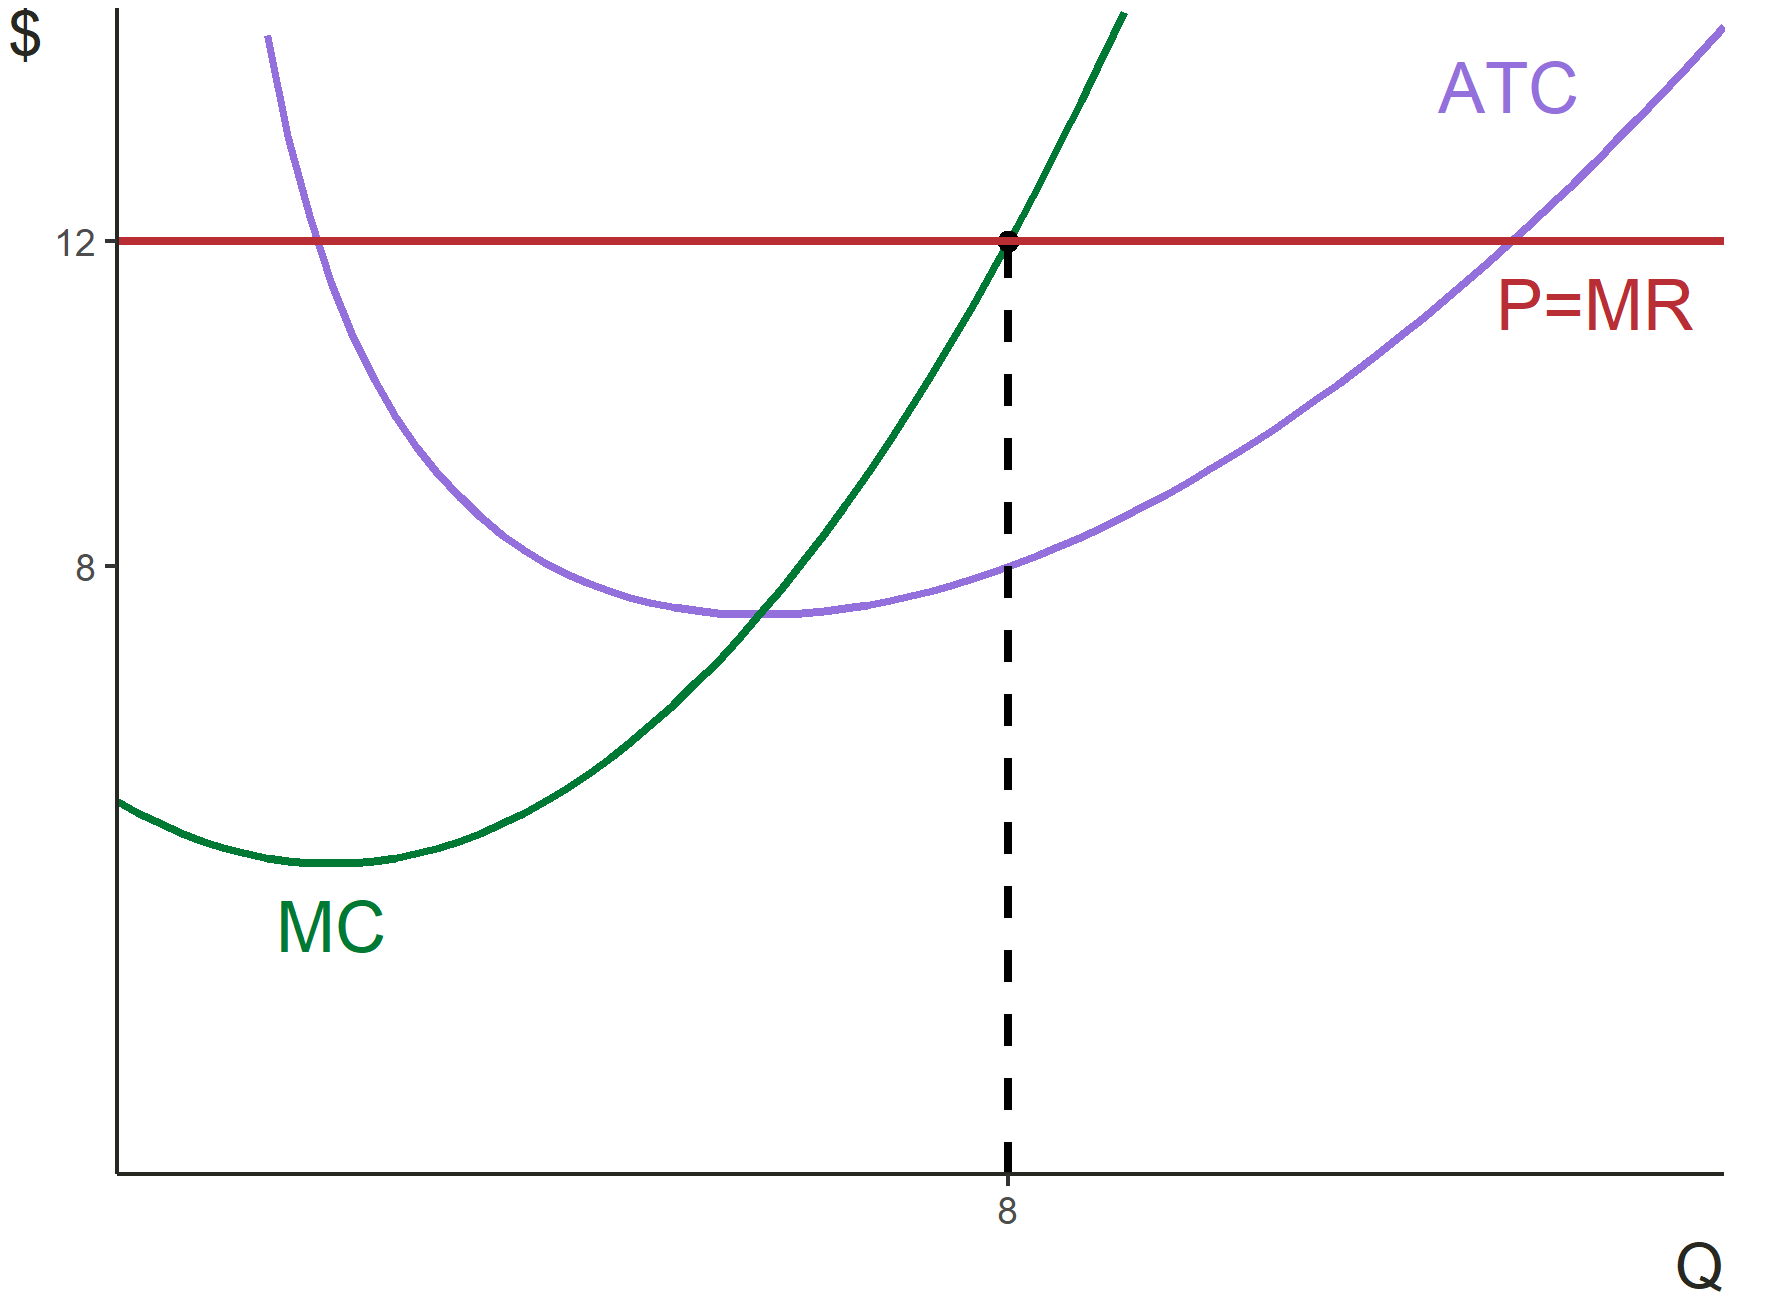
\includegraphics[width=8cm]{prod dec 1.png}
        \end{figure}
    \end{itemize}
\end{frame}

\begin{frame}{Visualizing Positive Profit for a PC Firm}
    \begin{itemize}[<+->]
        \item Since $\pi=(P-ATC)Q$, profit is given by the following box 
        \begin{figure}
            \centering
            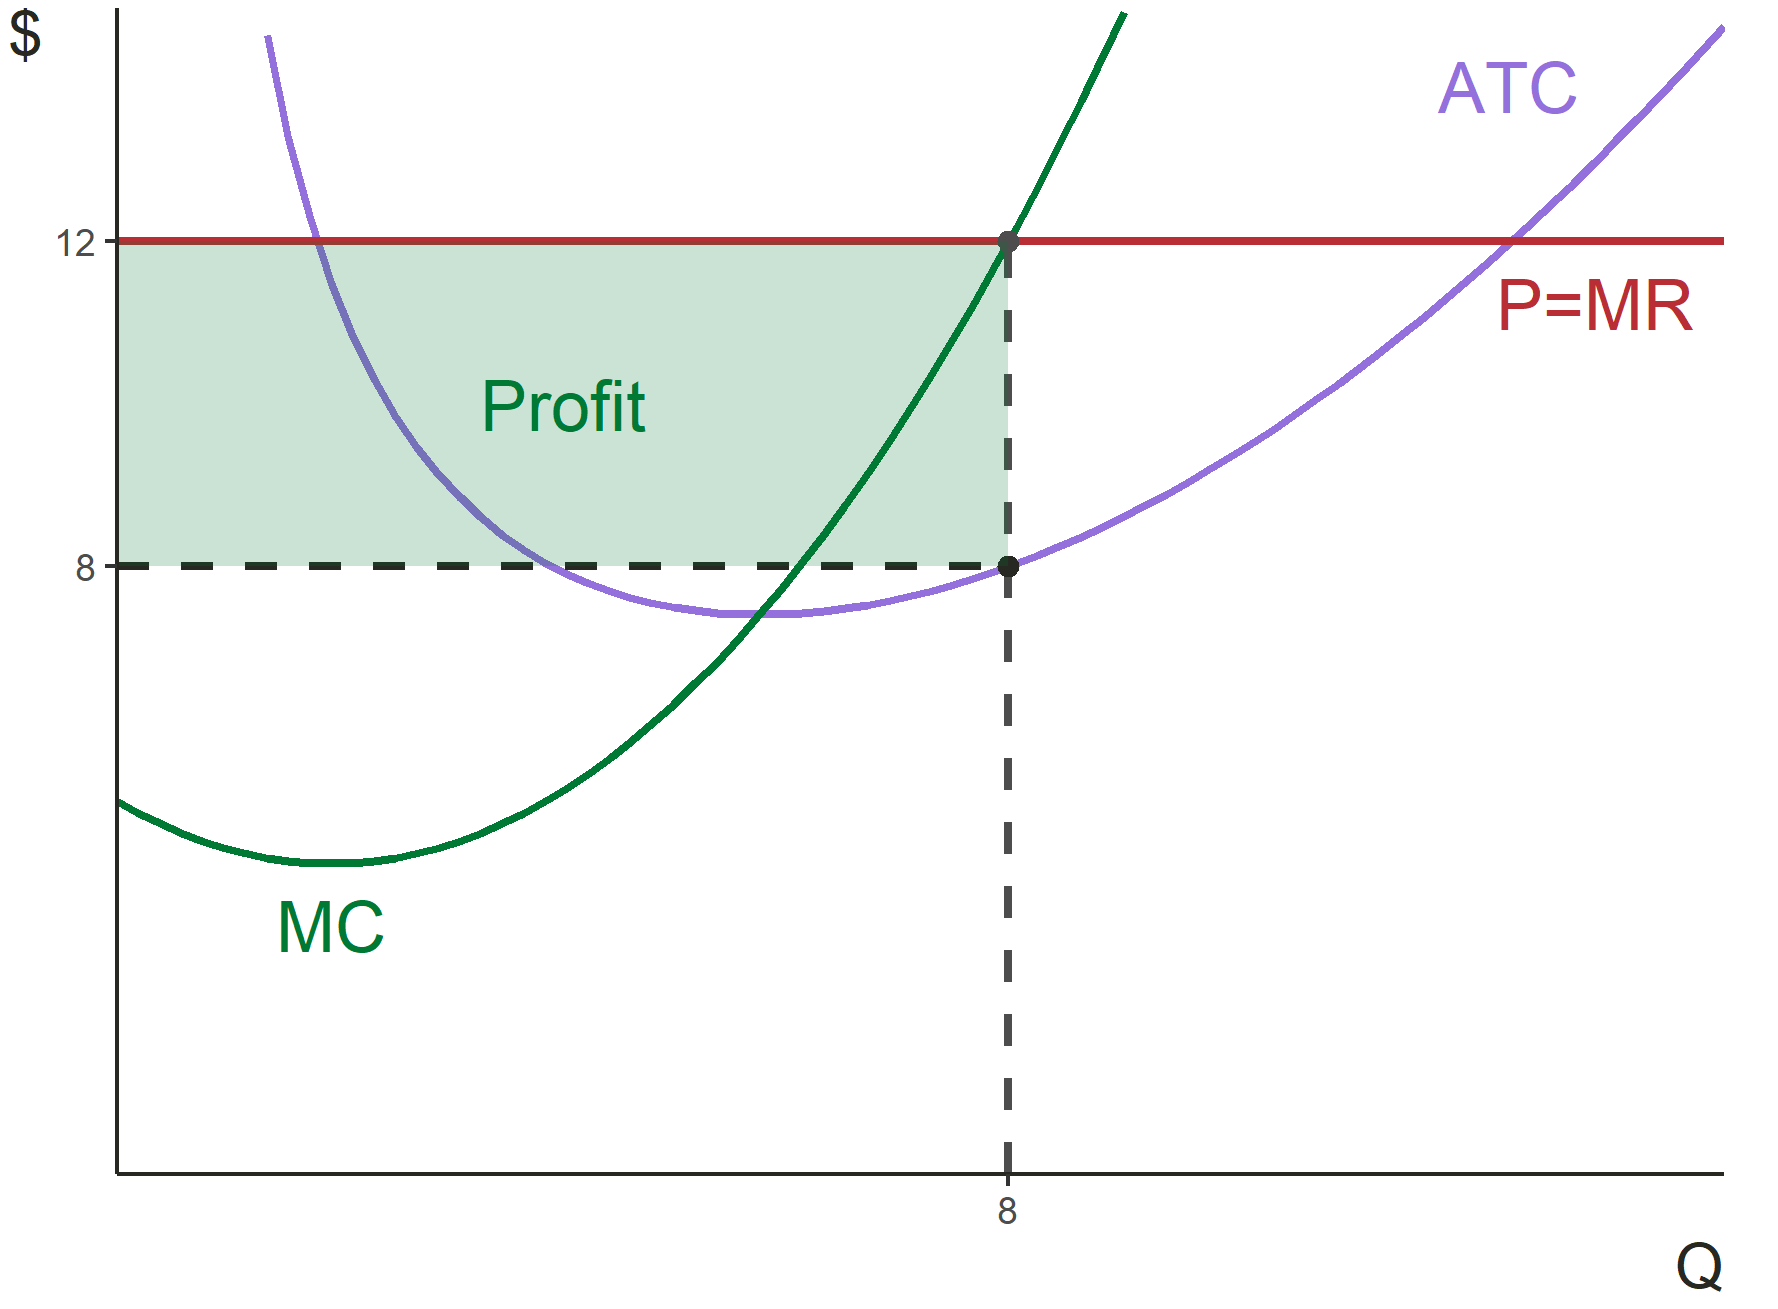
\includegraphics[width=8cm]{pmax1.png}
            \caption*{In this case, $\pi=8(12-8)=\$32$}
        \end{figure}
    \end{itemize}
\end{frame}

\begin{frame}{Visualizing Zero Profit for a PC Firm}
    \begin{itemize}[<+->]
        \item In this case, we produce at $P=MC$, and this induces $ATC$ to equal $P$, so we get a profit of 0: 
        \begin{figure}
            \centering
            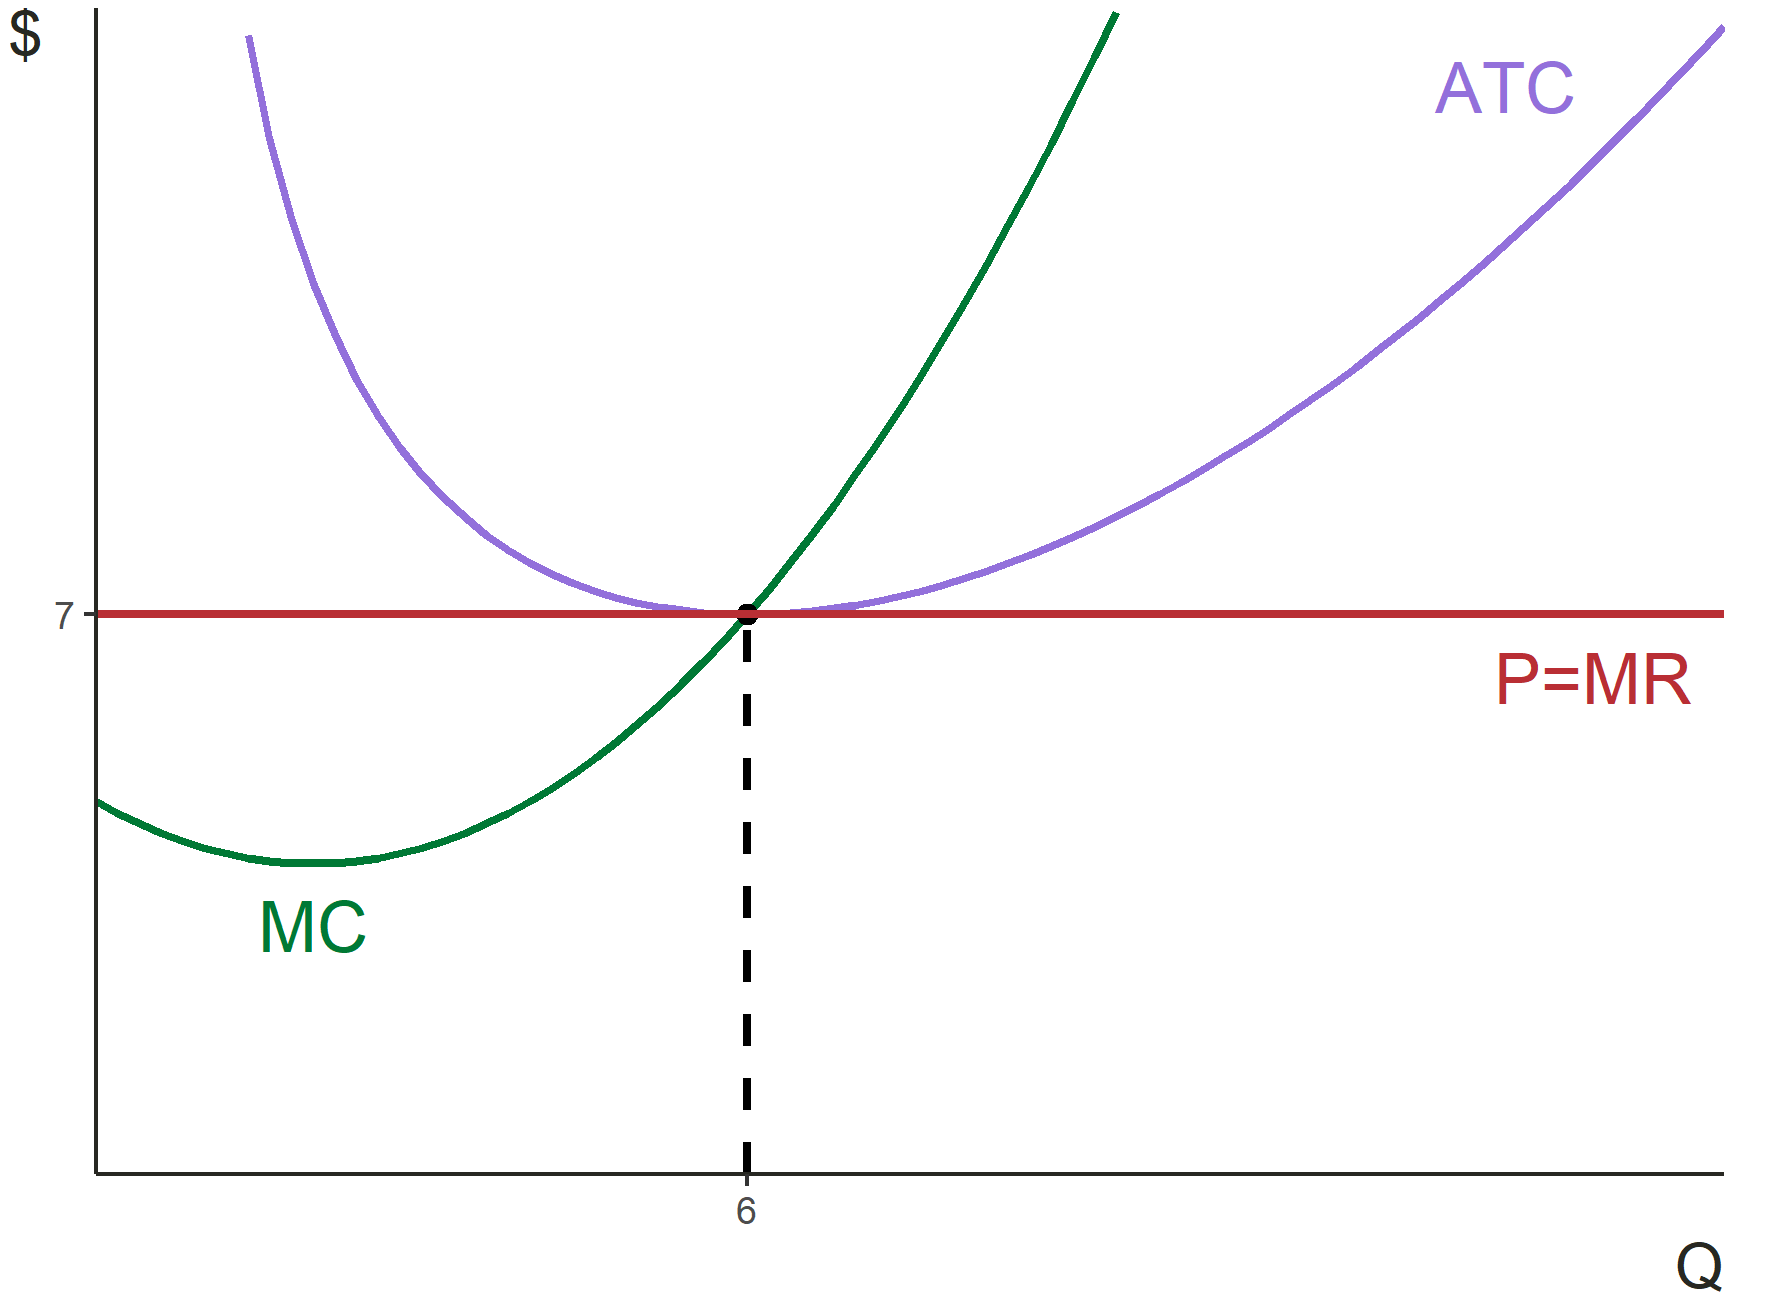
\includegraphics[width=8cm]{pmax2.png}
        \end{figure}
    \end{itemize}
\end{frame}

\begin{frame}{Visualizing Negative Profit for a PC Firm}
    \begin{itemize}[<+->]
        \item In this case, we produce at $P=MC$, and this induces $ATC$ to be below $P$, so we will make negative profit: 
        \begin{figure}
            \centering
            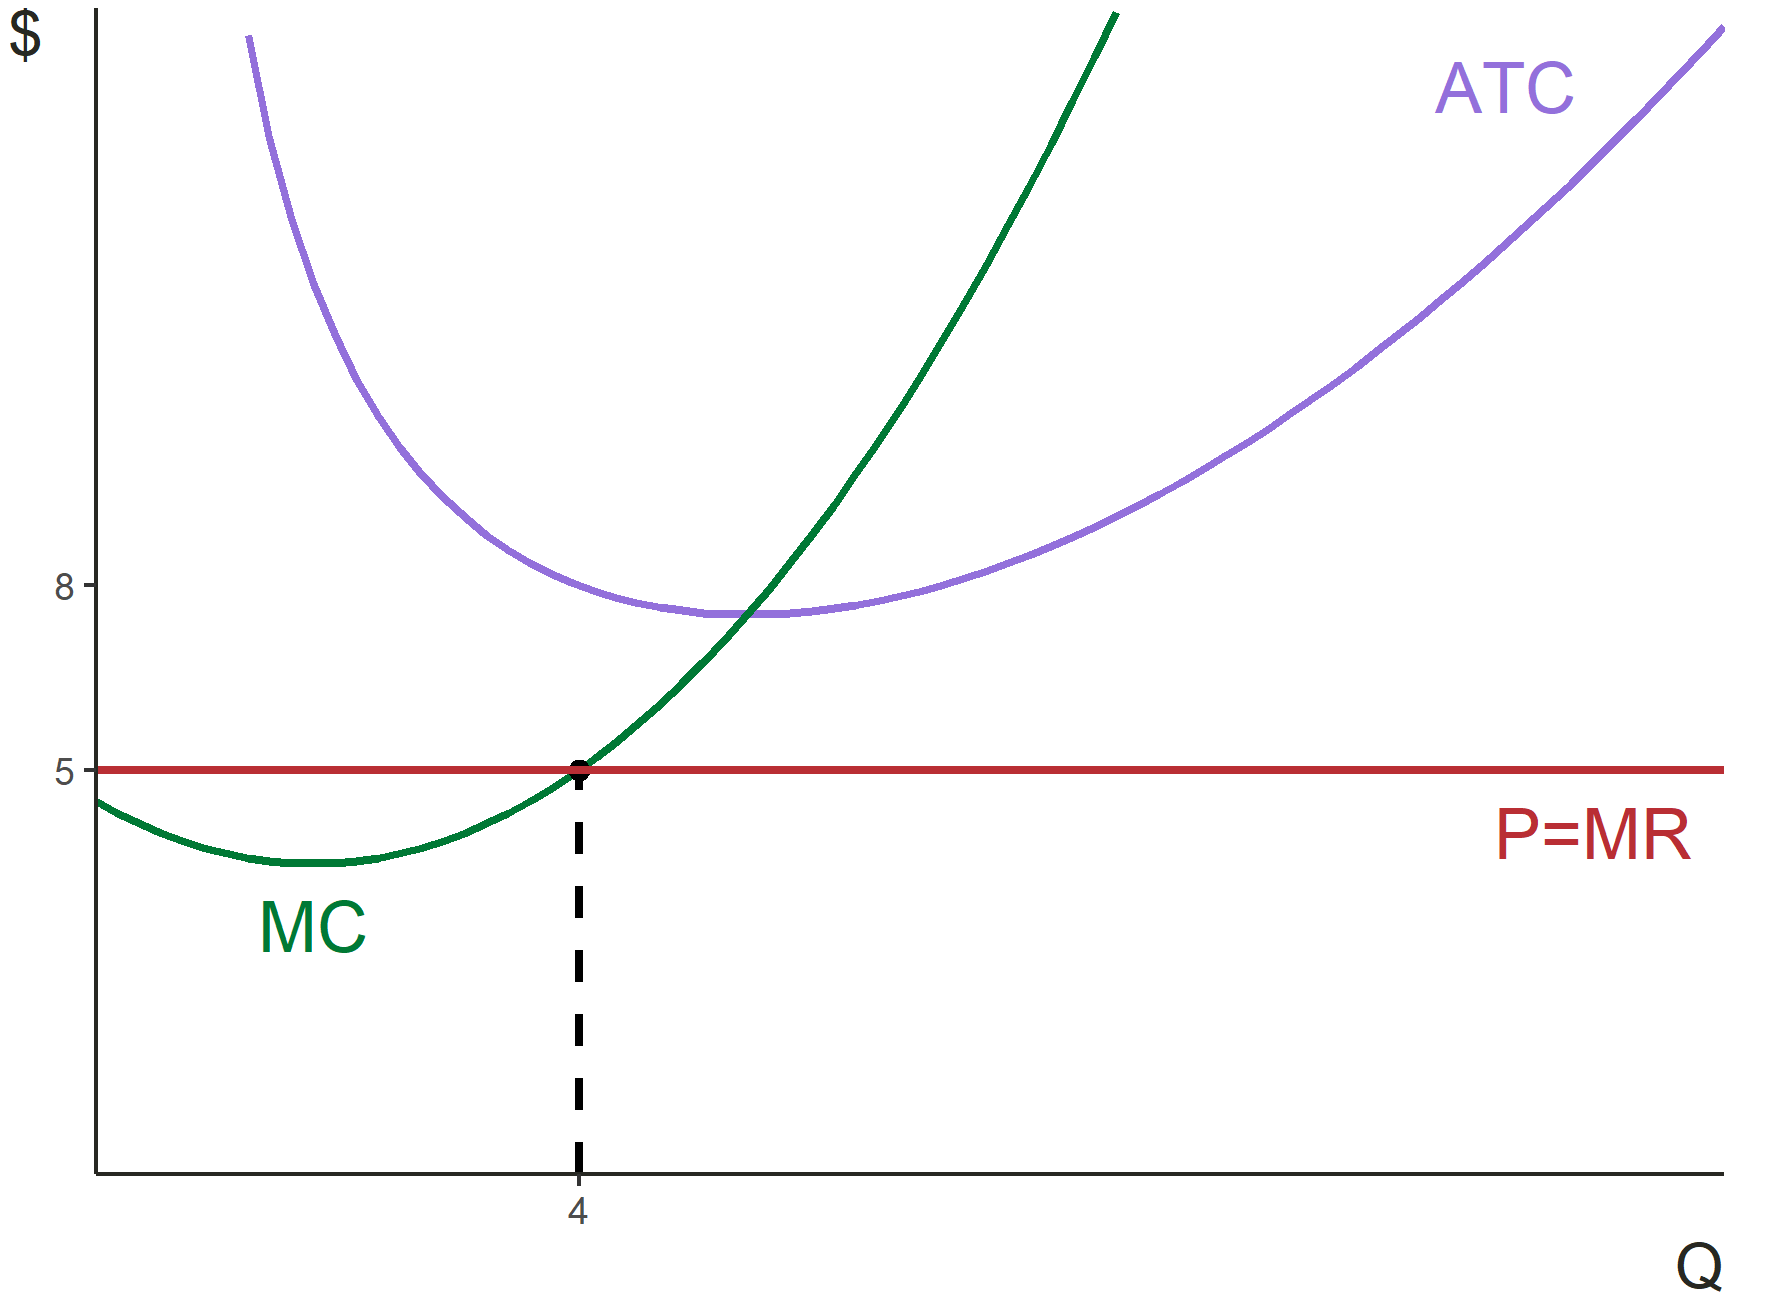
\includegraphics[width=8cm]{prod dec 3.png}
        \end{figure}
    \end{itemize}
\end{frame}

\begin{frame}{Visualizing Negative Profit for a PC Firm}
    \begin{itemize}[<+->]
        \item Specifically, we make $\pi=4(5-8)=-12$ 
        \begin{figure}
            \centering
            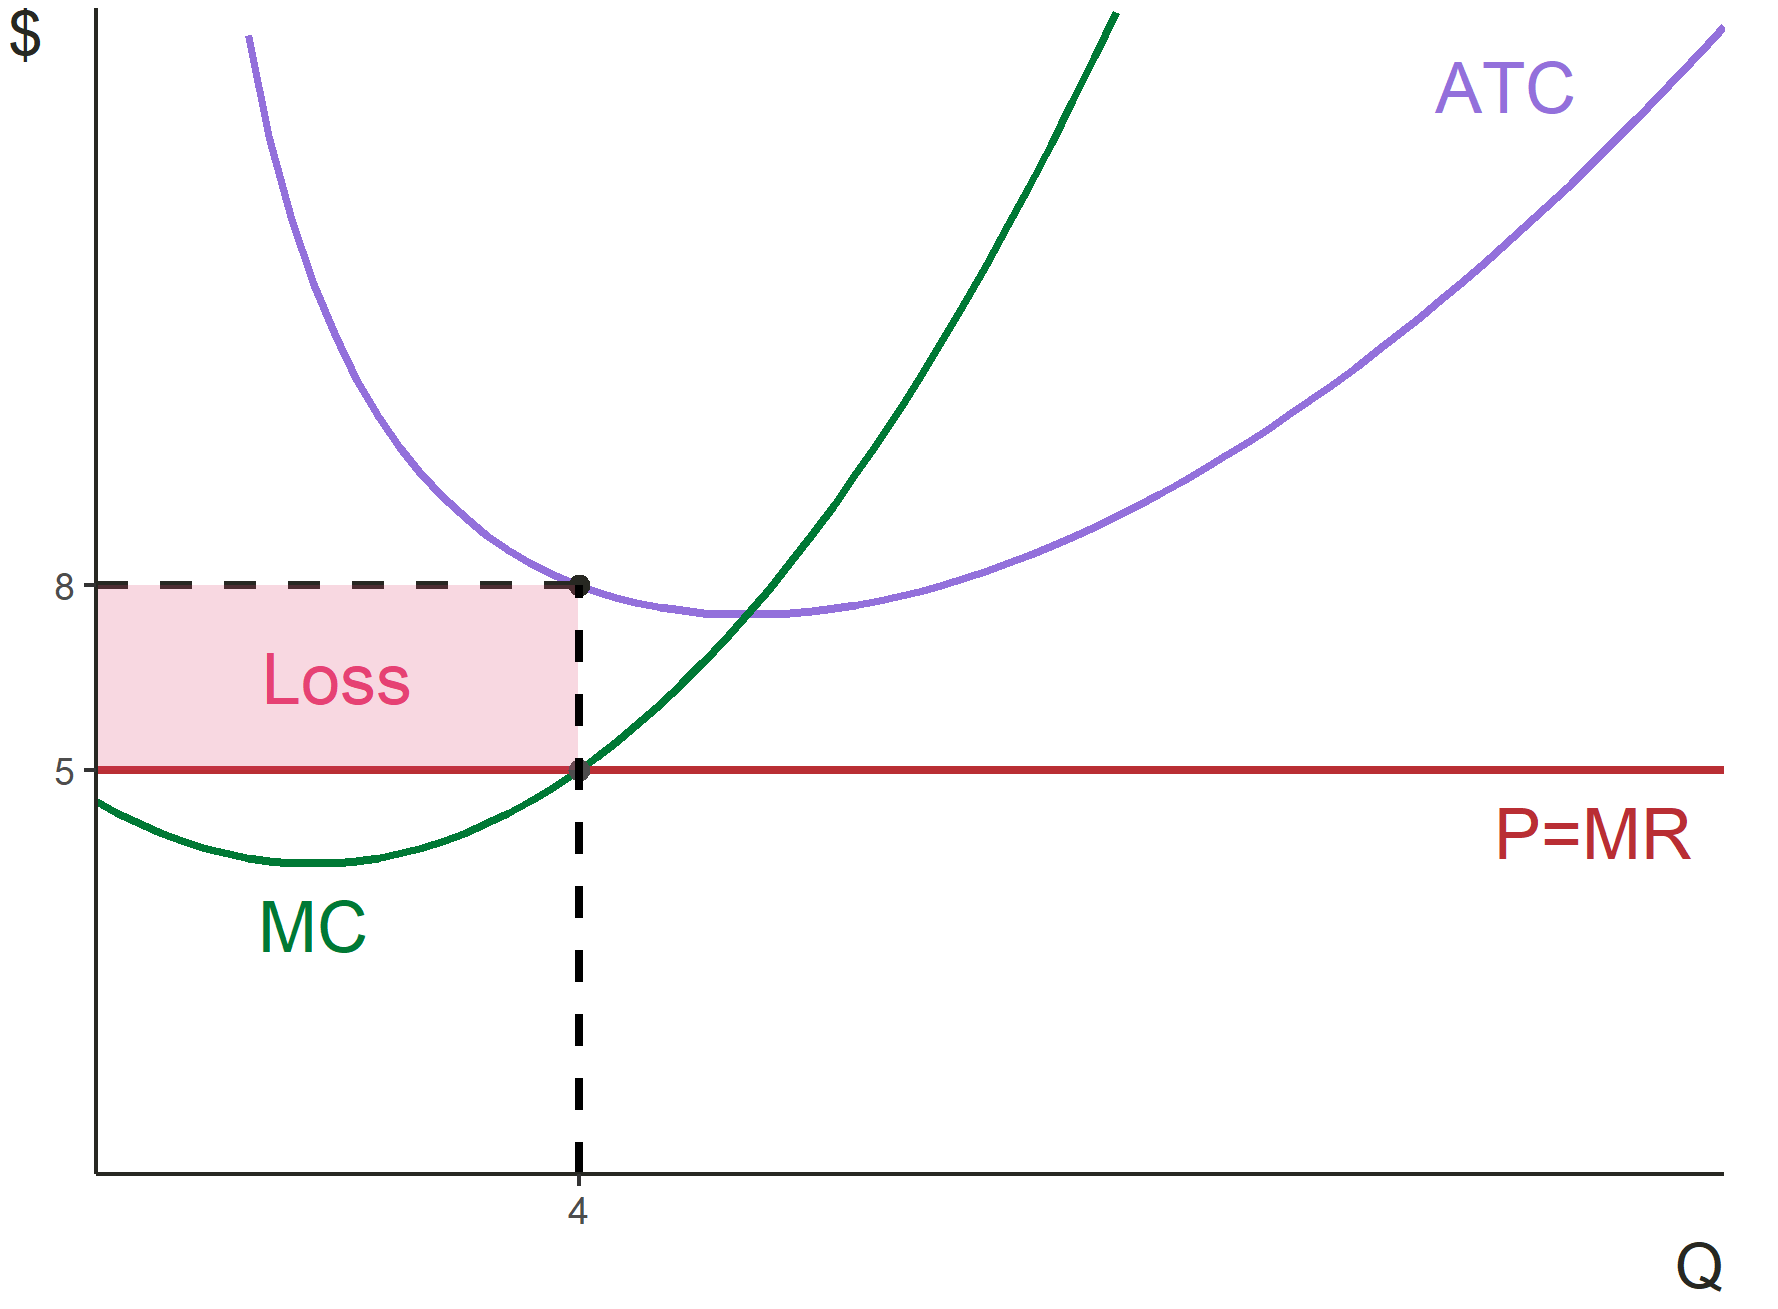
\includegraphics[width=8cm]{pmax3.png}
        \end{figure}
    \end{itemize}
\end{frame}

\begin{frame}{Visualizing Profit for a PC Firm}
    \begin{itemize}[<+->]
        \item Note: Based on the shape on MC, we can see that if $MC<MR$, the firm should increase production. If $MC>MR$, the firm should decrease production. If $MR=MC$, the firm should produce at that level
        \begin{figure}
            \centering
            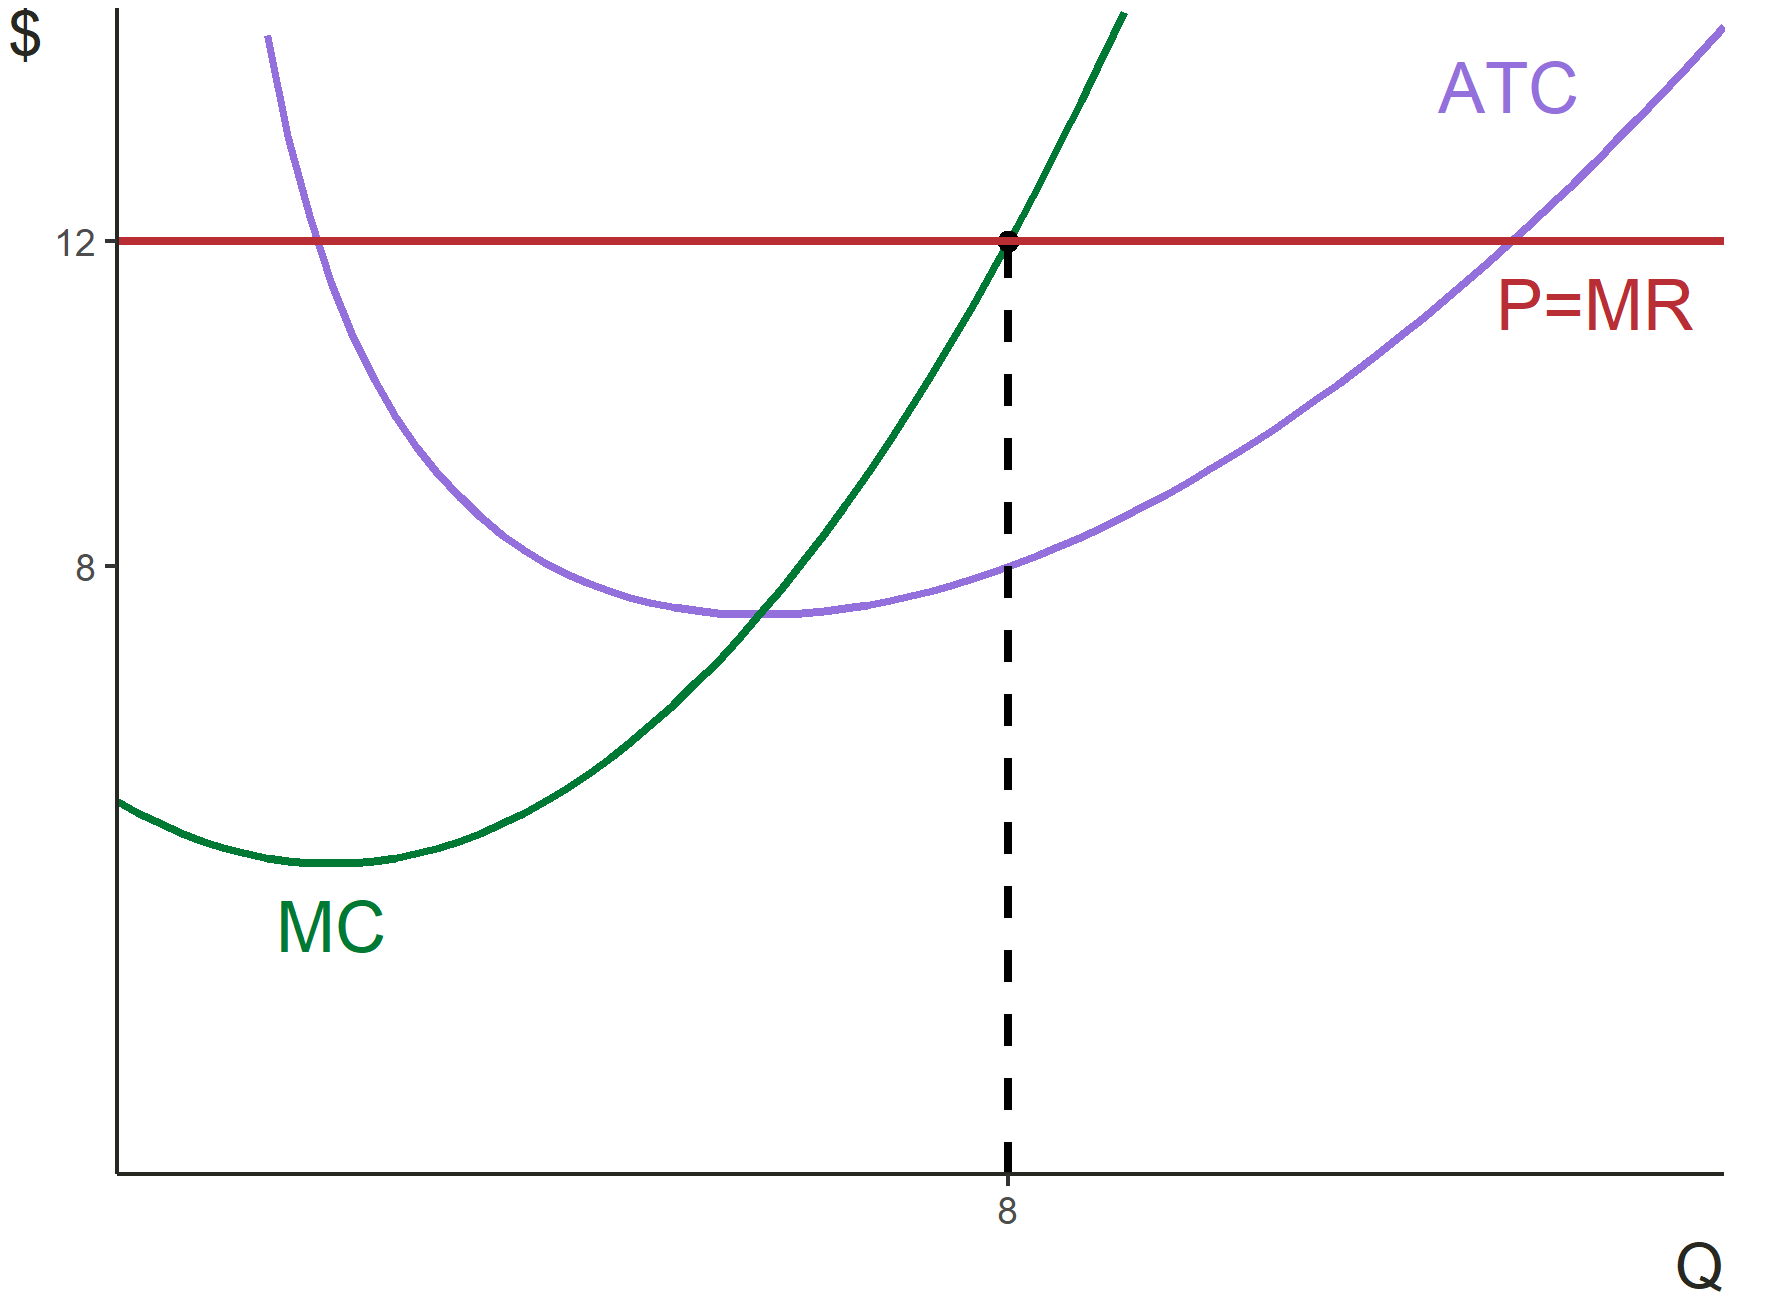
\includegraphics[width=7cm]{prod dec 1.png}
        \end{figure}
    \end{itemize}
\end{frame}

\section*{Shutting Down}

\begin{frame}{Should I Stay in Business?}
    \begin{itemize}[<+->]
        \item Suppose I started a restaurant one year ago, with
        \begin{itemize}
            \item Monthly revenue of $\$10,000$
            \item Monthly ingredients costing of $\$2,000$ and monthly labor costing $\$5,000$
            \item Fixed cost $\$120,000$ to start up the business
        \end{itemize}
        \item How much yearly profit am I making?
        \begin{itemize}
            \item $\pi=(12)10k-(12)7k-120k=-84k$
        \end{itemize}
        \item I lost $\$84,000$ this year! Should I shut down!?
    \end{itemize}
\end{frame}

\begin{frame}{Should I Stay in Business?}
    \begin{itemize}[<+->]
        \item No
        \begin{itemize}
            \item I am making $10k-7k=\$3k$ every month, discounting the startup costs of my business
            \item Therefore, I am making $\$36k$ a year. In less than 4 years, I will have paid off my startup costs and will be making positive profit
        \end{itemize}
    \end{itemize}
\end{frame}

\begin{frame}{Should this PC Firm Shut Down?}
    \begin{itemize}[<+->]
        \item This firm is earning negative profit. Should they shut down?
        \begin{figure}
            \centering
            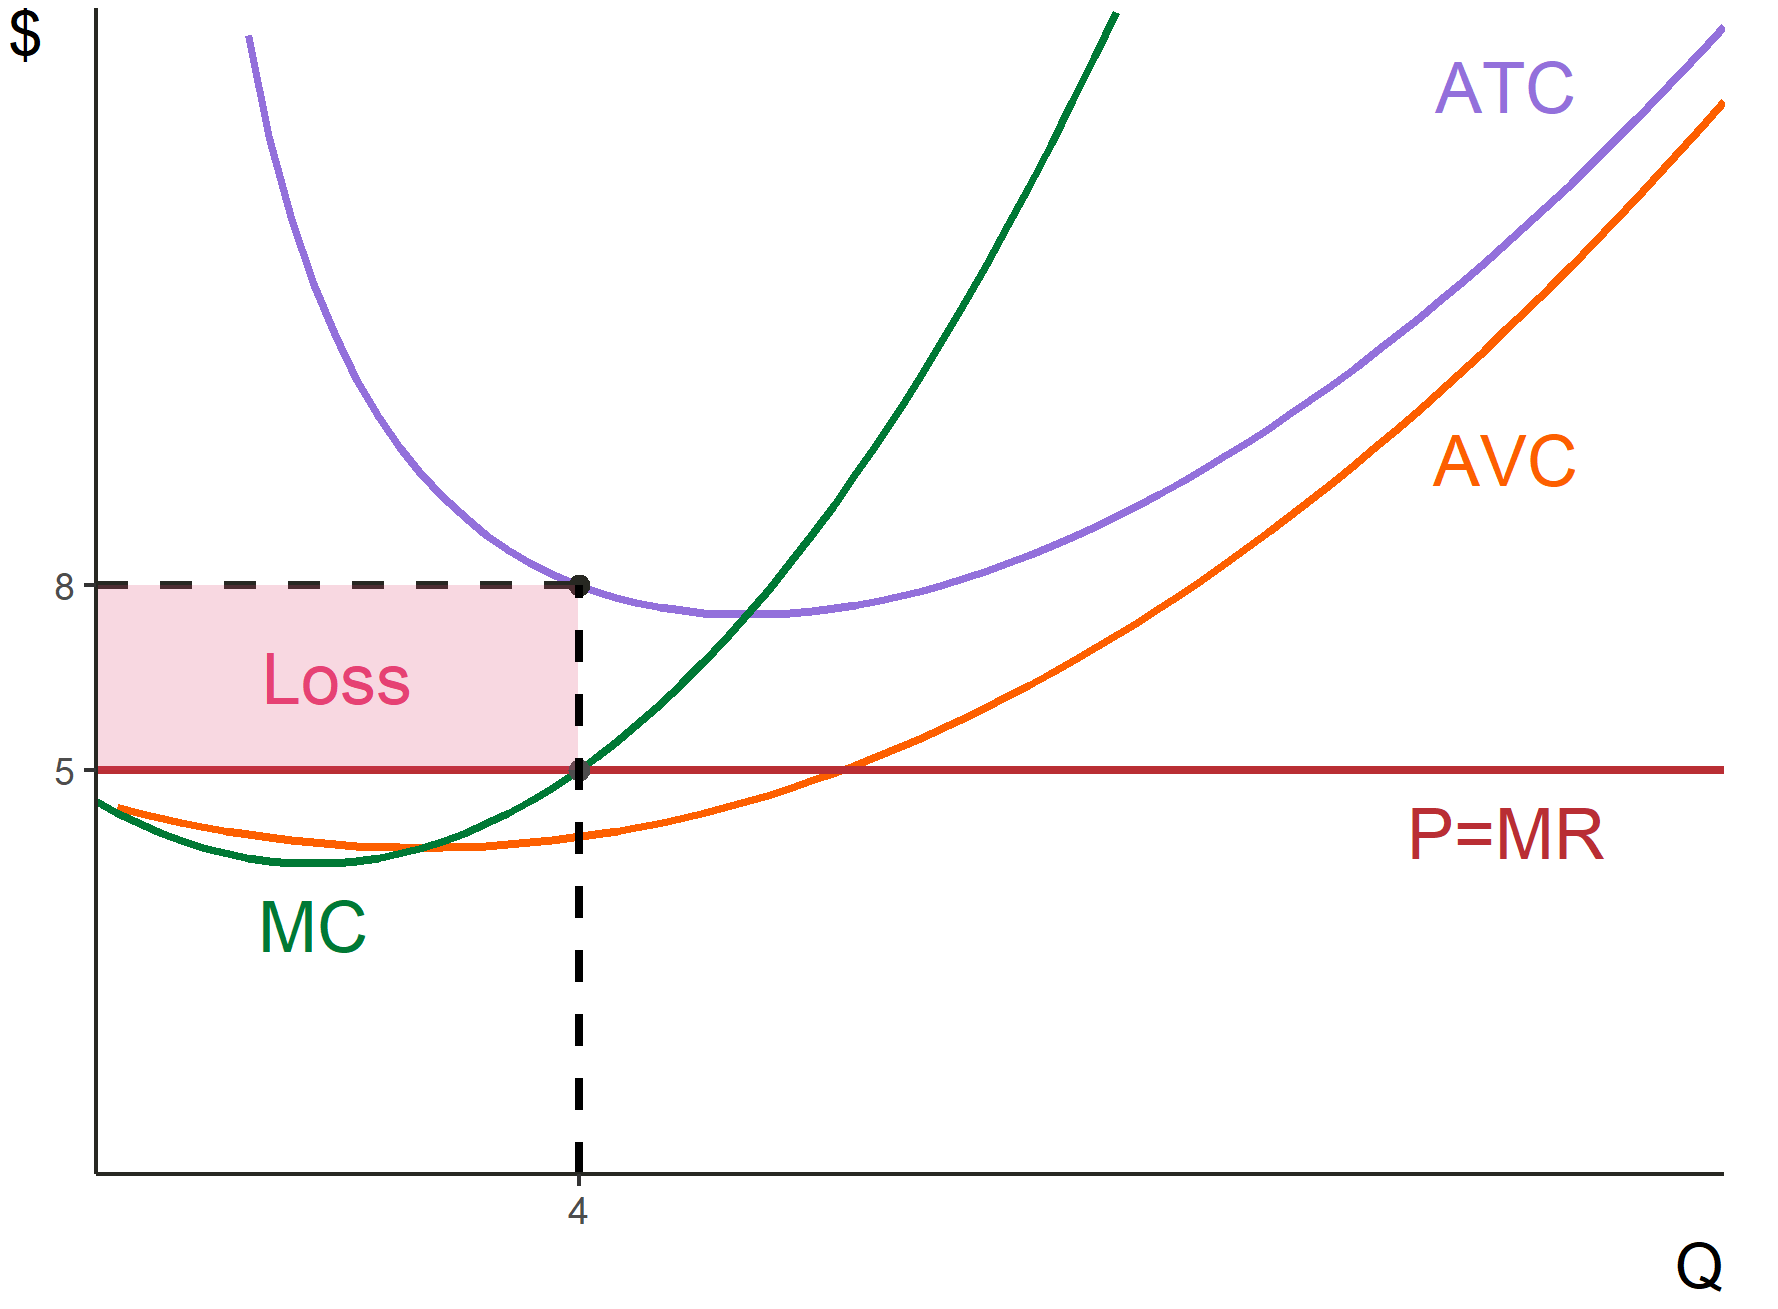
\includegraphics[width=8cm]{shutdown question.png}
        \end{figure}
    \end{itemize}
\end{frame}

\begin{frame}{Should this PC Firm Shut Down?}
    \begin{itemize}[<+->]
        \item No!
        \begin{itemize}
            \item This is the same story that I just told, visually (and with different numbers)
        \end{itemize}
    \end{itemize}
\end{frame}

\begin{frame}{Shutdown Condition in the Short Run}
    \begin{itemize}[<+->]
        \item So when should I shut down?
        \begin{itemize}
            \item In the short run, I should stay in business as long as I cover my variable costs \textit{on average}
            \item That is, as long as my \underline{average} total revenue is greater than or equal to my \underline{average} variable cost, I shouldn't shut down
            \item Note that average revenue is equal to $AR=\frac{TR}{Q}=\frac{P\cdot Q}{Q}=P$
            \item Therefore, I should stay in business so long as the price exceeds $AVC$
        \end{itemize}
        \item Conclusion: in the short run, the firm will shut down as long as 
        $$P>\min(AVC)$$
        where the $\min(AVC)$ is the minimum value that AVC attains for $Q>0$ (i.e., in the positive quadrant)
    \end{itemize}
\end{frame}

\begin{frame}{P and AVC}
    \begin{itemize}[<+->]
        \item The book says shutdown when $P<AVC$
        \item But $P$ is a horizontal line, and $AVC$ is a parabola:
        \begin{figure}
            \centering
            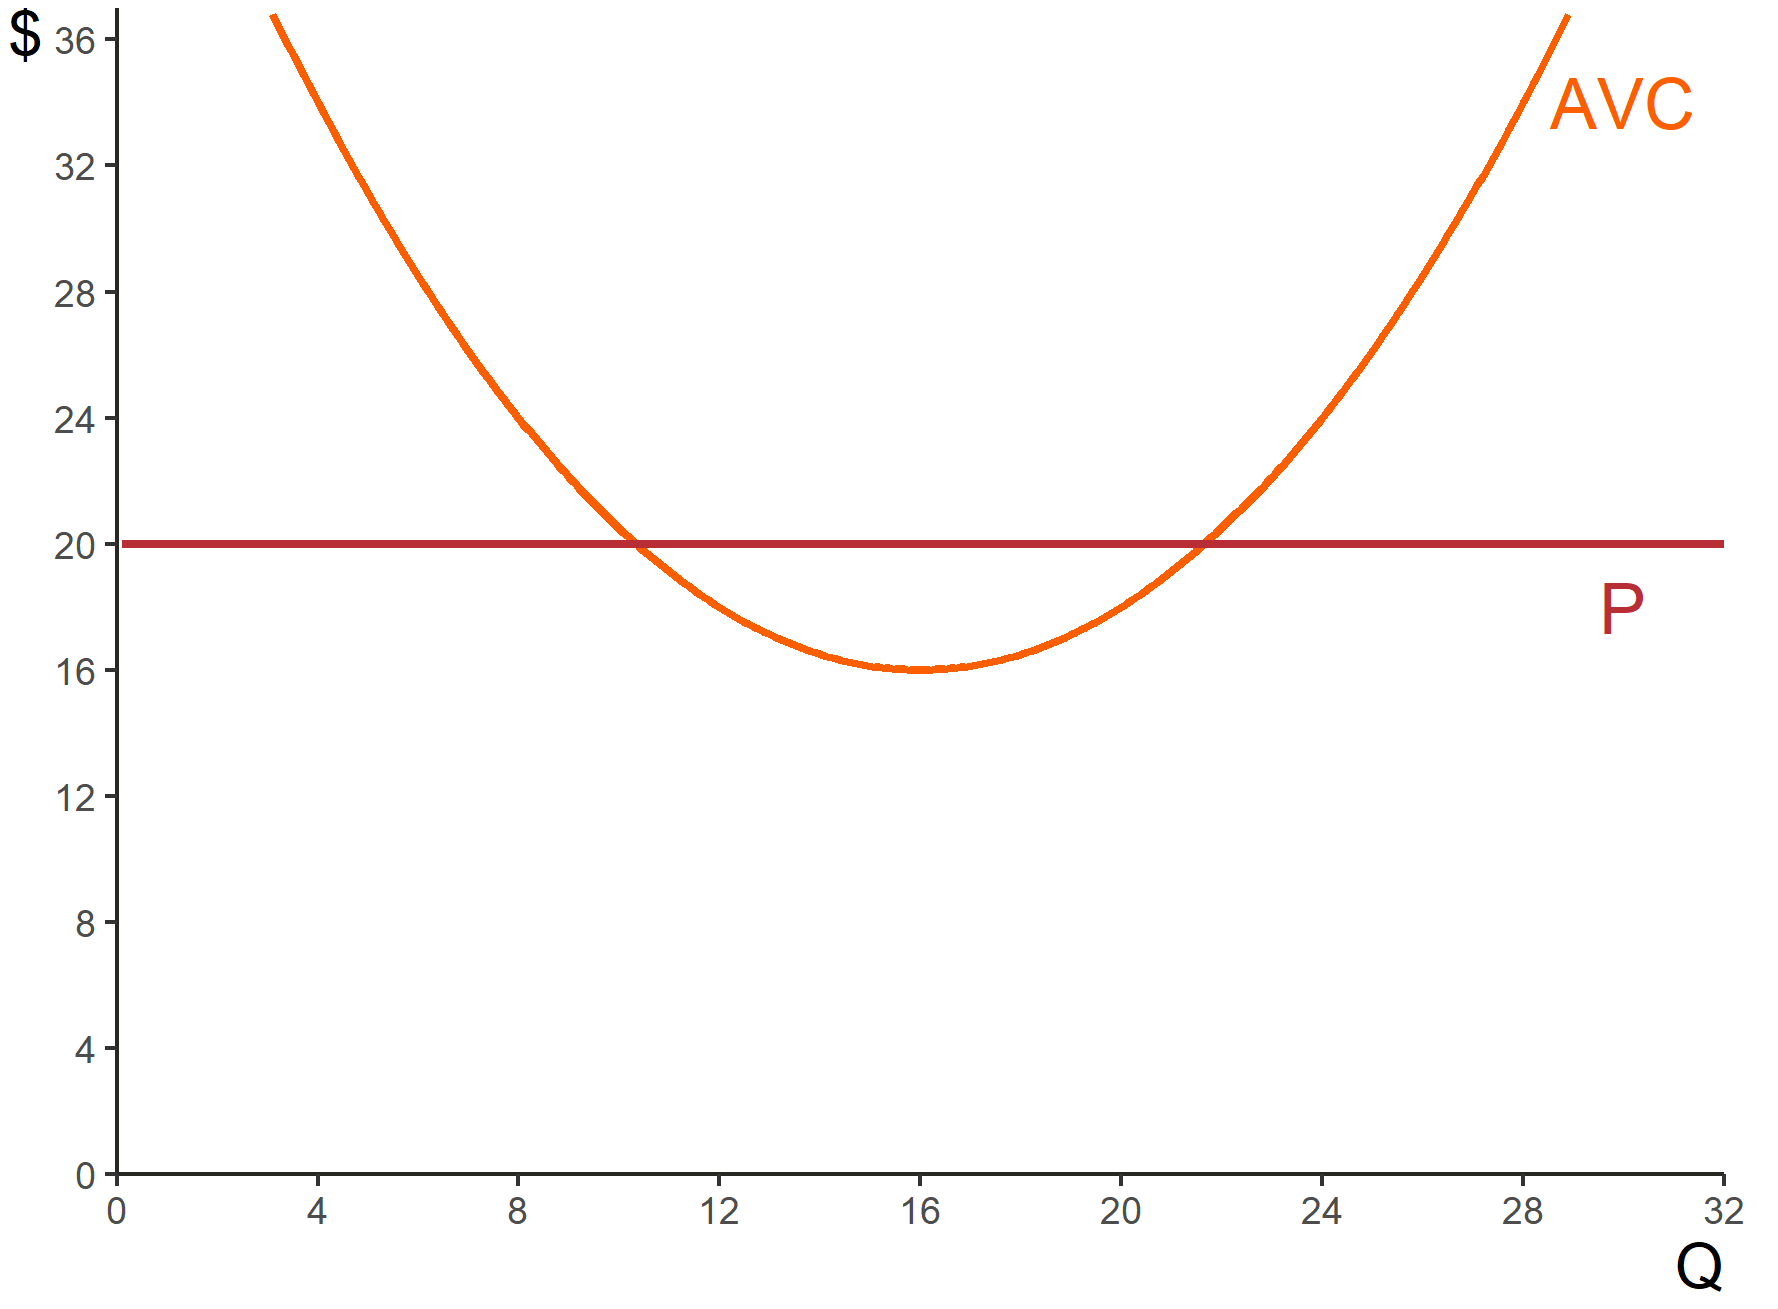
\includegraphics[width=7cm]{bad shut.png}
        \end{figure}
        \item There are many places where $P>AVC$, and many where $P<AVC$
    \end{itemize}
\end{frame}

\begin{frame}{Precise Shutdown Condition}
    \begin{itemize}[<+->]
        \item More precisely, we should shut down when $P<\min(AVC)$; i.e., when the $P$ line is completely below $AVC$
        \begin{figure}
            \centering
            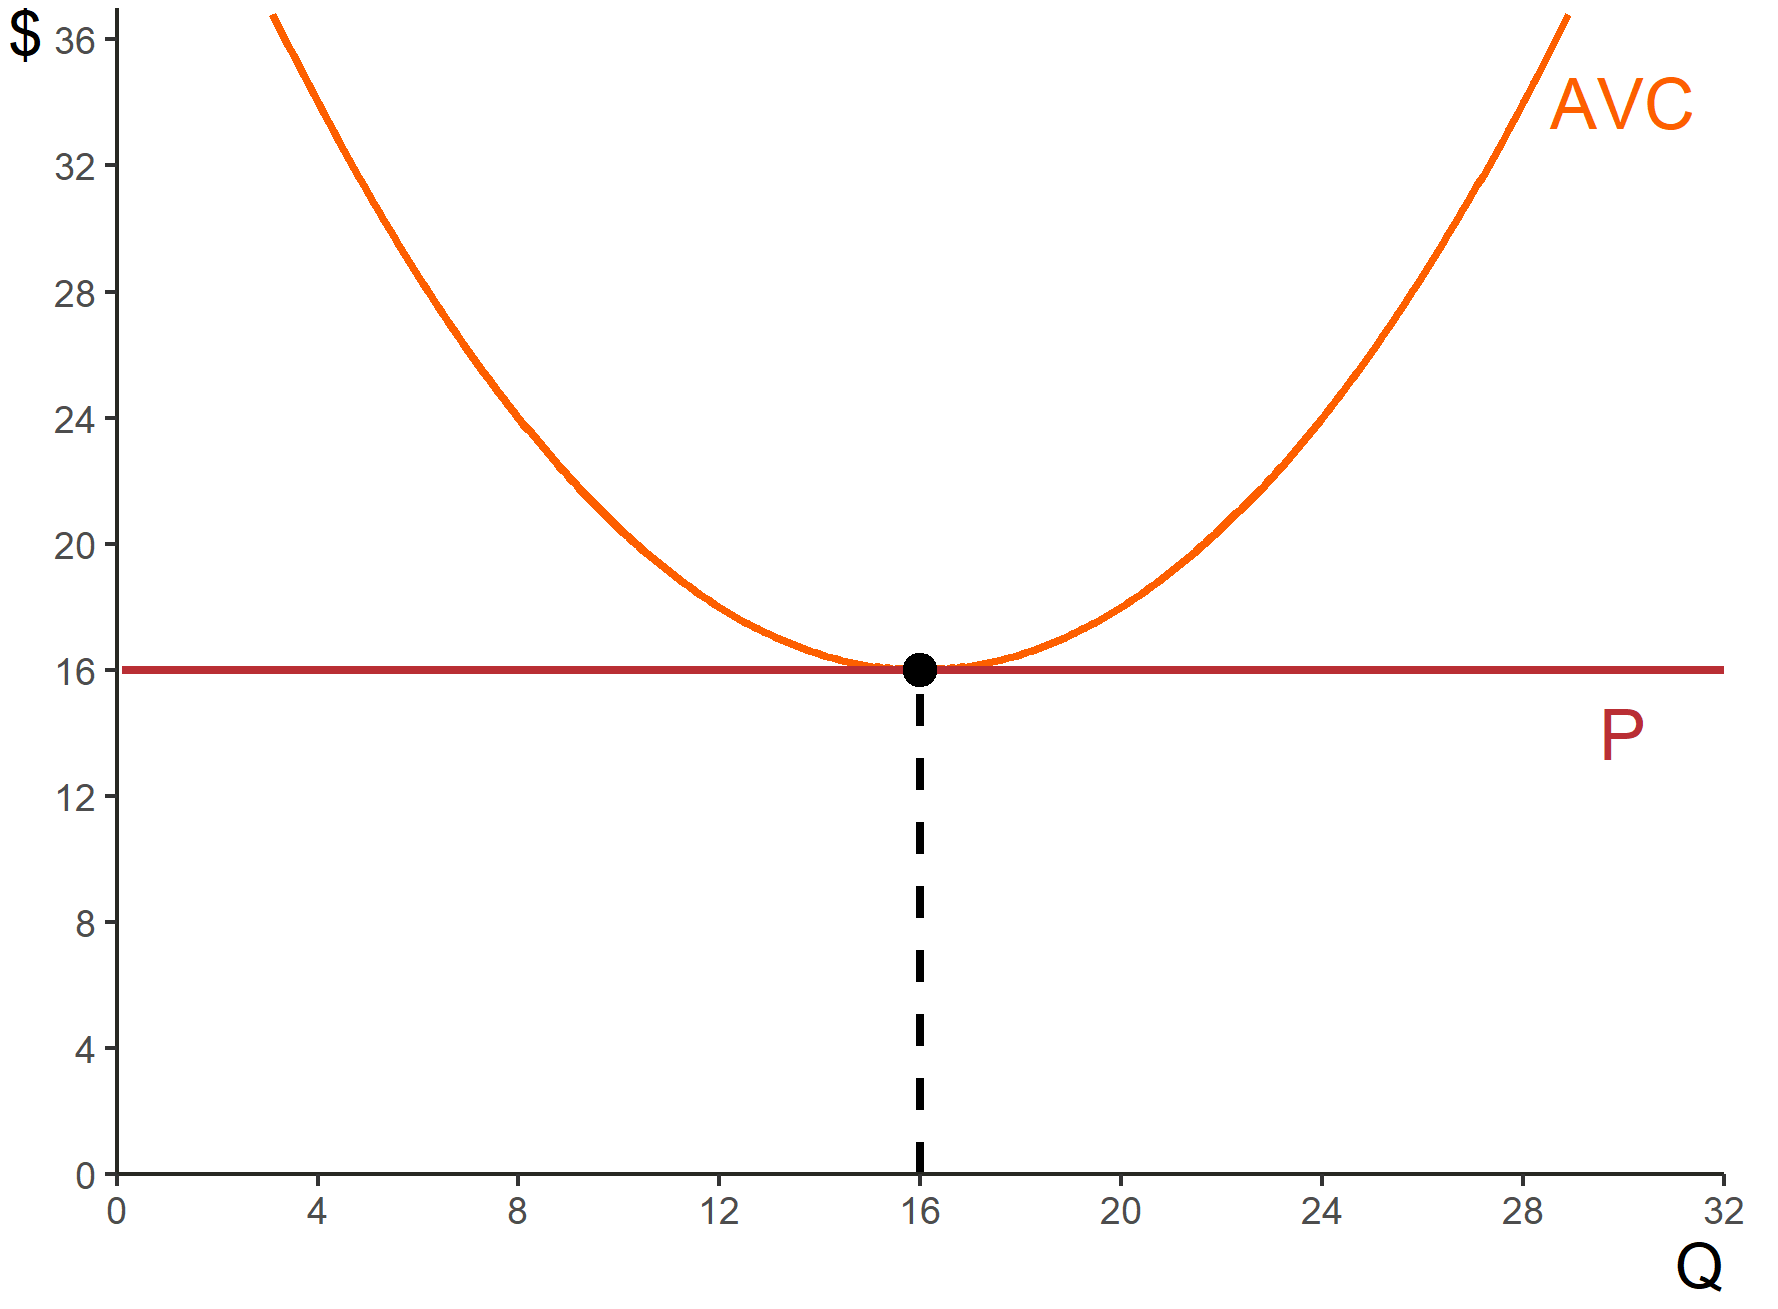
\includegraphics[width=7cm]{good shut.png}
        \end{figure}
        %\item Note: this is implicitly based on where MC intersects AVC, but we don't need to worry about that
    \end{itemize}
\end{frame}

\begin{frame}{Should We Shutdown 1}
    \begin{itemize}[<+->]
        \item Should this firm shut down? Are they making profit?
        \begin{figure}
            \centering
            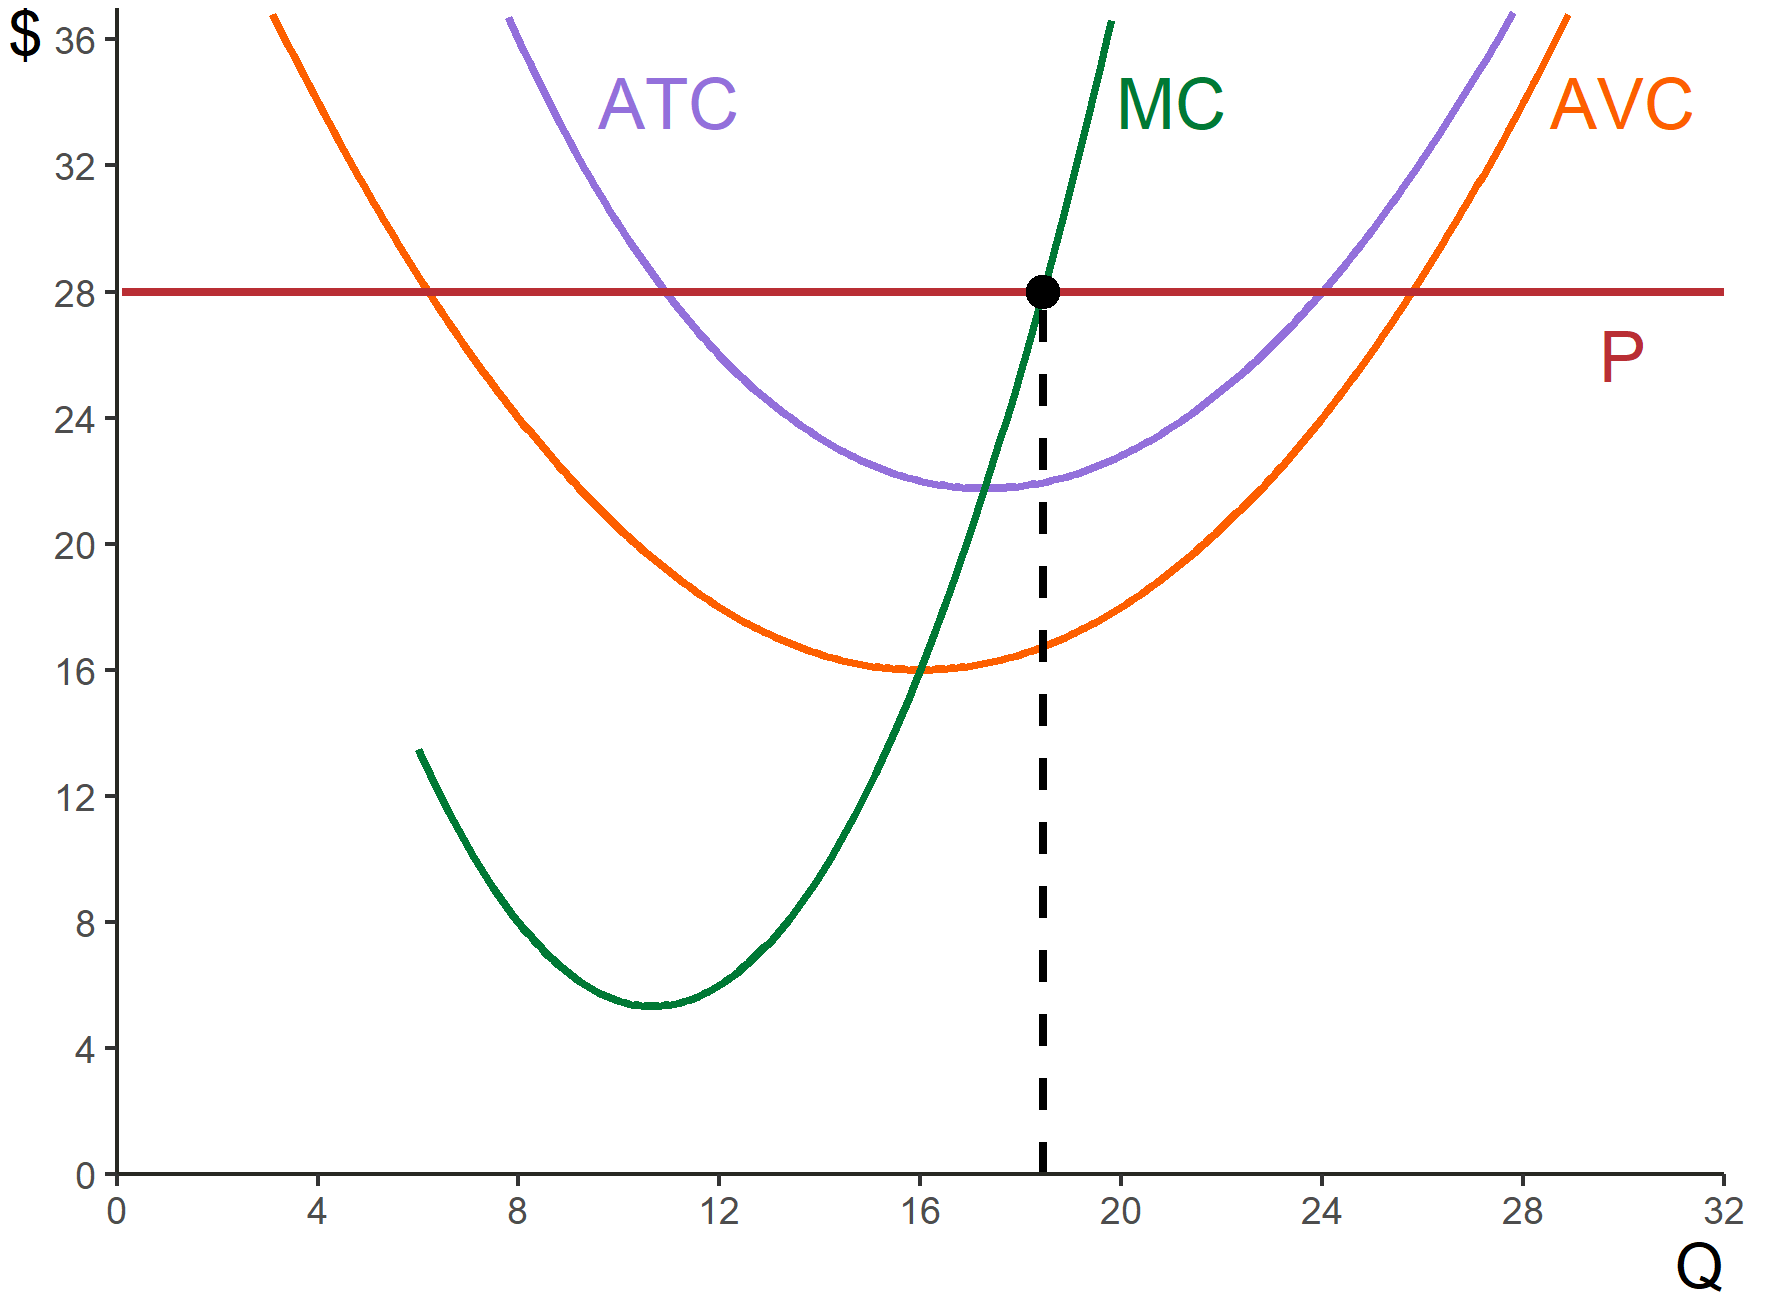
\includegraphics[width=7cm]{shut ex1.png}
        \end{figure}
        \item No, they are making positive profit
    \end{itemize}
\end{frame}

\begin{frame}{Should We Shutdown 2}
    \begin{itemize}[<+->]
        \item Should this firm shut down? Are they making profit?
        \begin{figure}
            \centering
            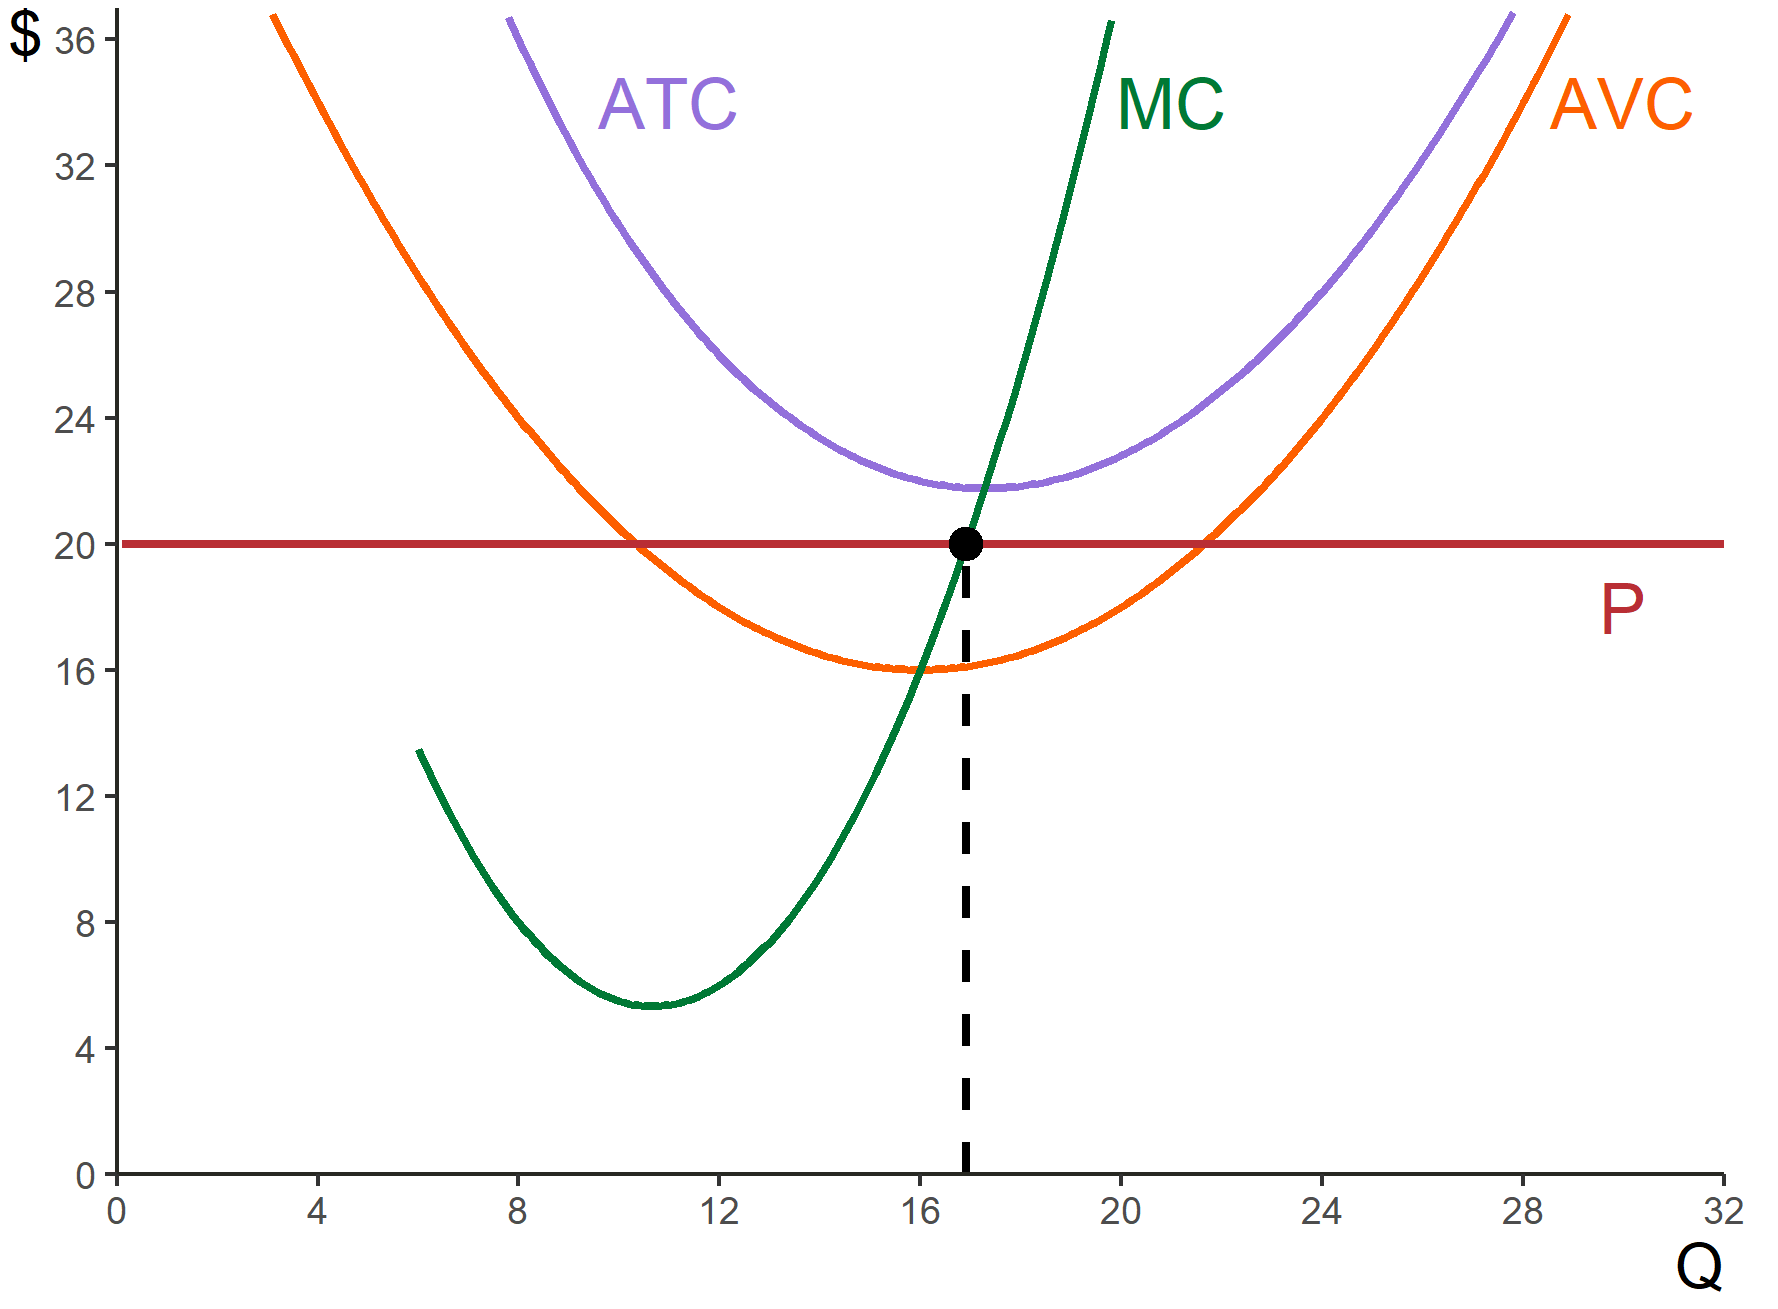
\includegraphics[width=7cm]{shut ex2.png}
        \end{figure}
        \item No, they are making negative profit but covering their variable costs on average
    \end{itemize}
\end{frame}

\begin{frame}{Should We Shutdown 3}
    \begin{itemize}[<+->]
        \item Should this firm shut down? Are they making profit?
        \begin{figure}
            \centering
            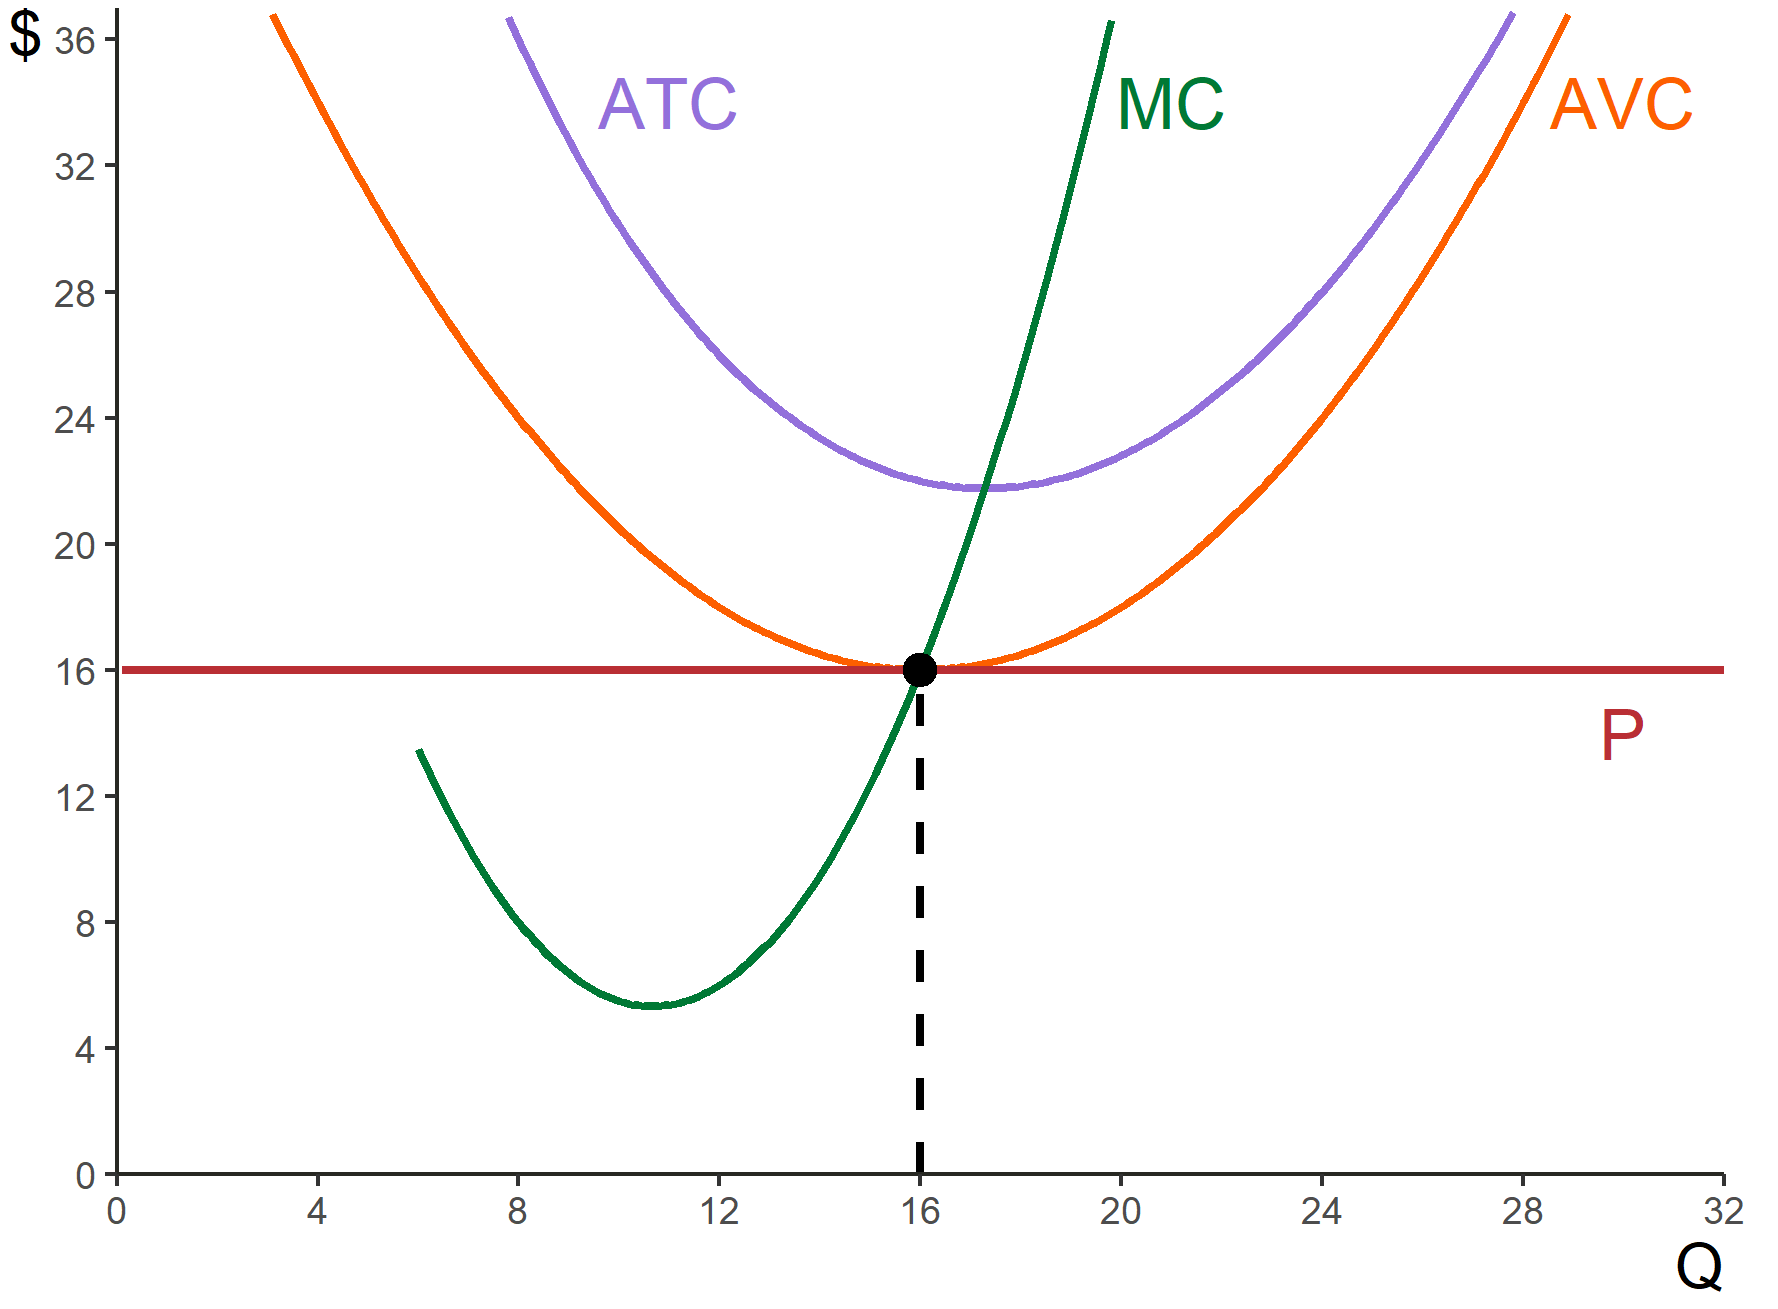
\includegraphics[width=7cm]{shut ex3.png}
        \end{figure}
        \item Yes/no, they are perfectly breaking even on their variable costs
    \end{itemize}
\end{frame}

\begin{frame}{Should We Shutdown 4}
    \begin{itemize}[<+->]
        \item Should this firm shut down? Are they making profit?
        \begin{figure}
            \centering
            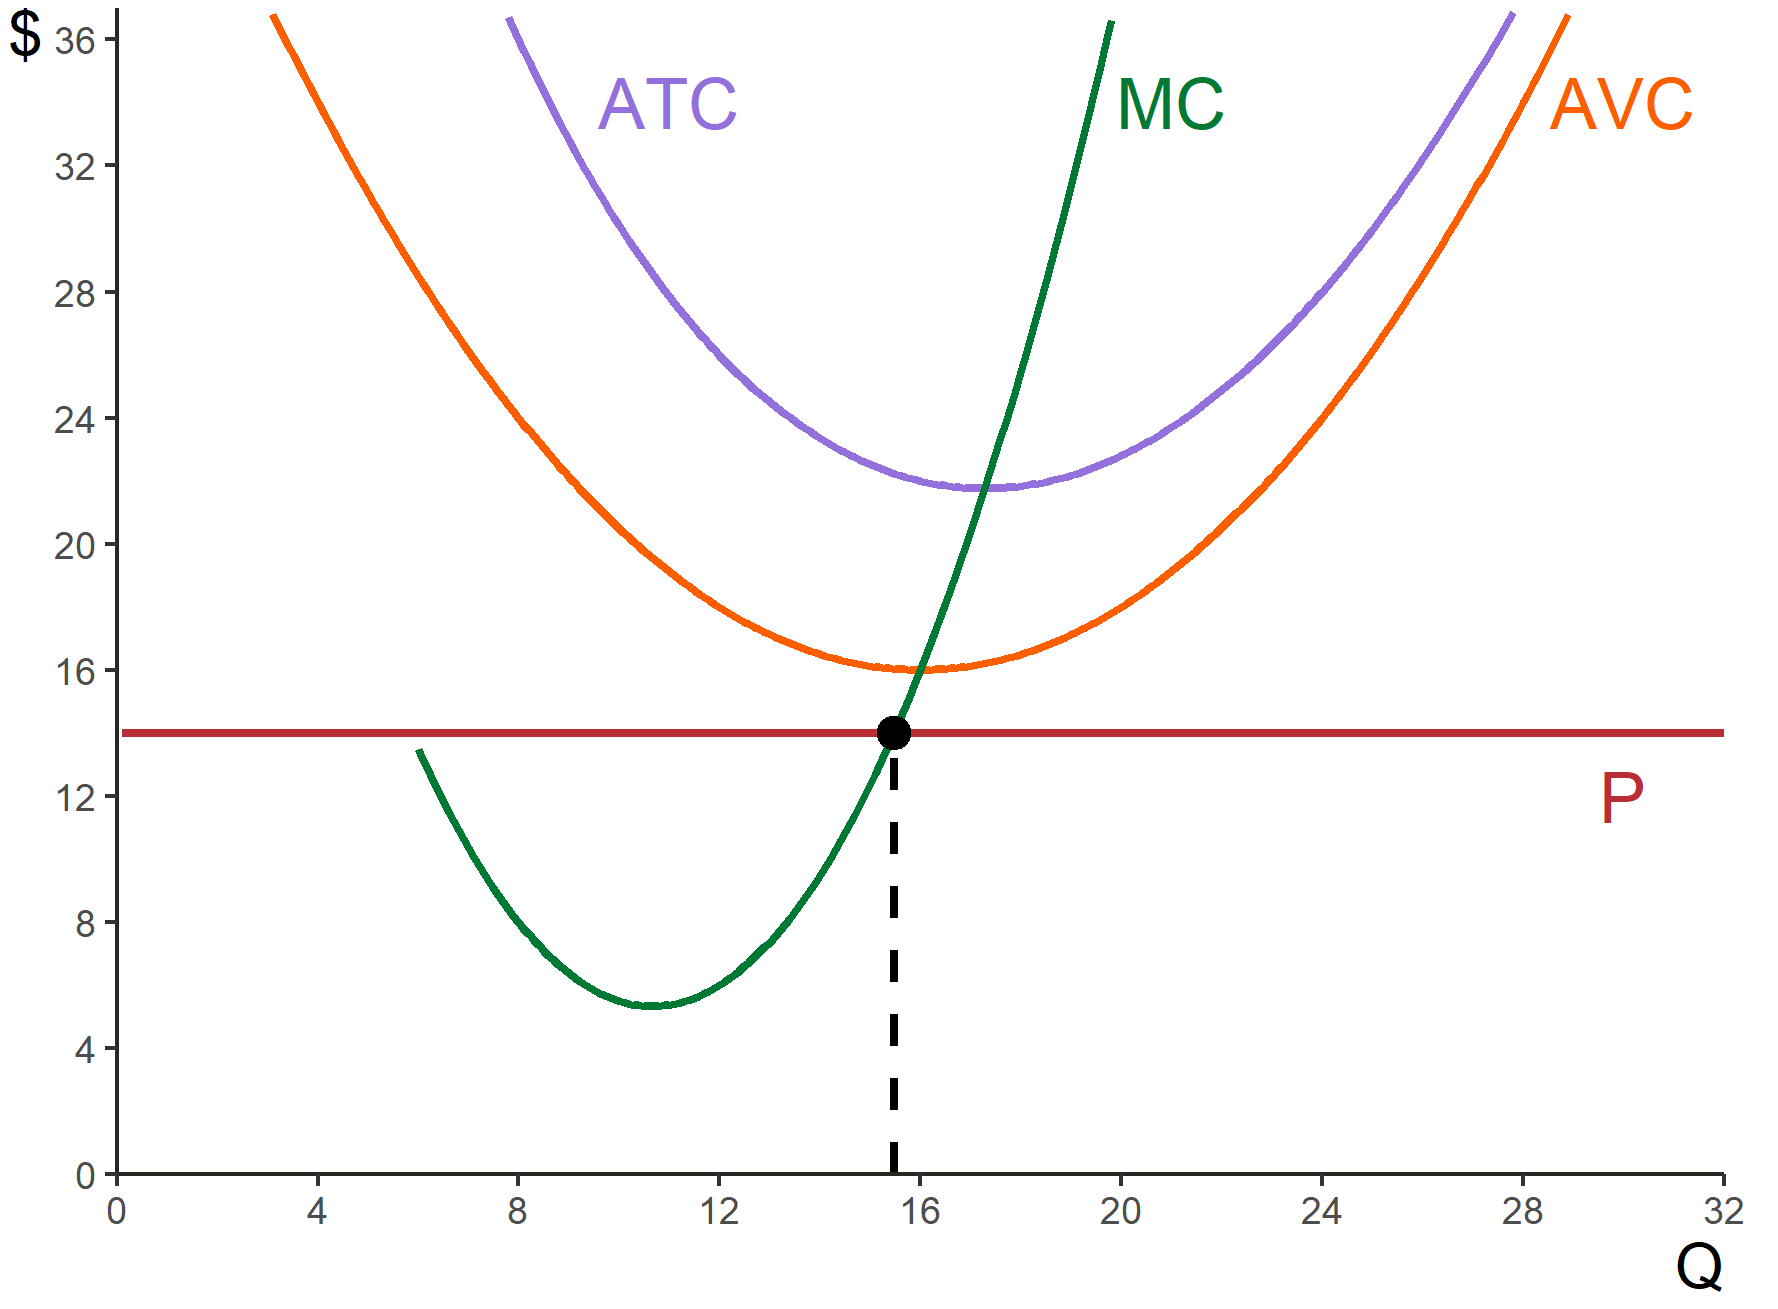
\includegraphics[width=7cm]{shut ex4.png}
        \end{figure}
        \item Yes, they are not covering their variable costs on average
    \end{itemize}
\end{frame}

\begin{frame}{Full Shutdown Picture}
    \begin{itemize}[<+->]
        \item This summarizes the full shutdown picture
        \begin{figure}
            \centering
            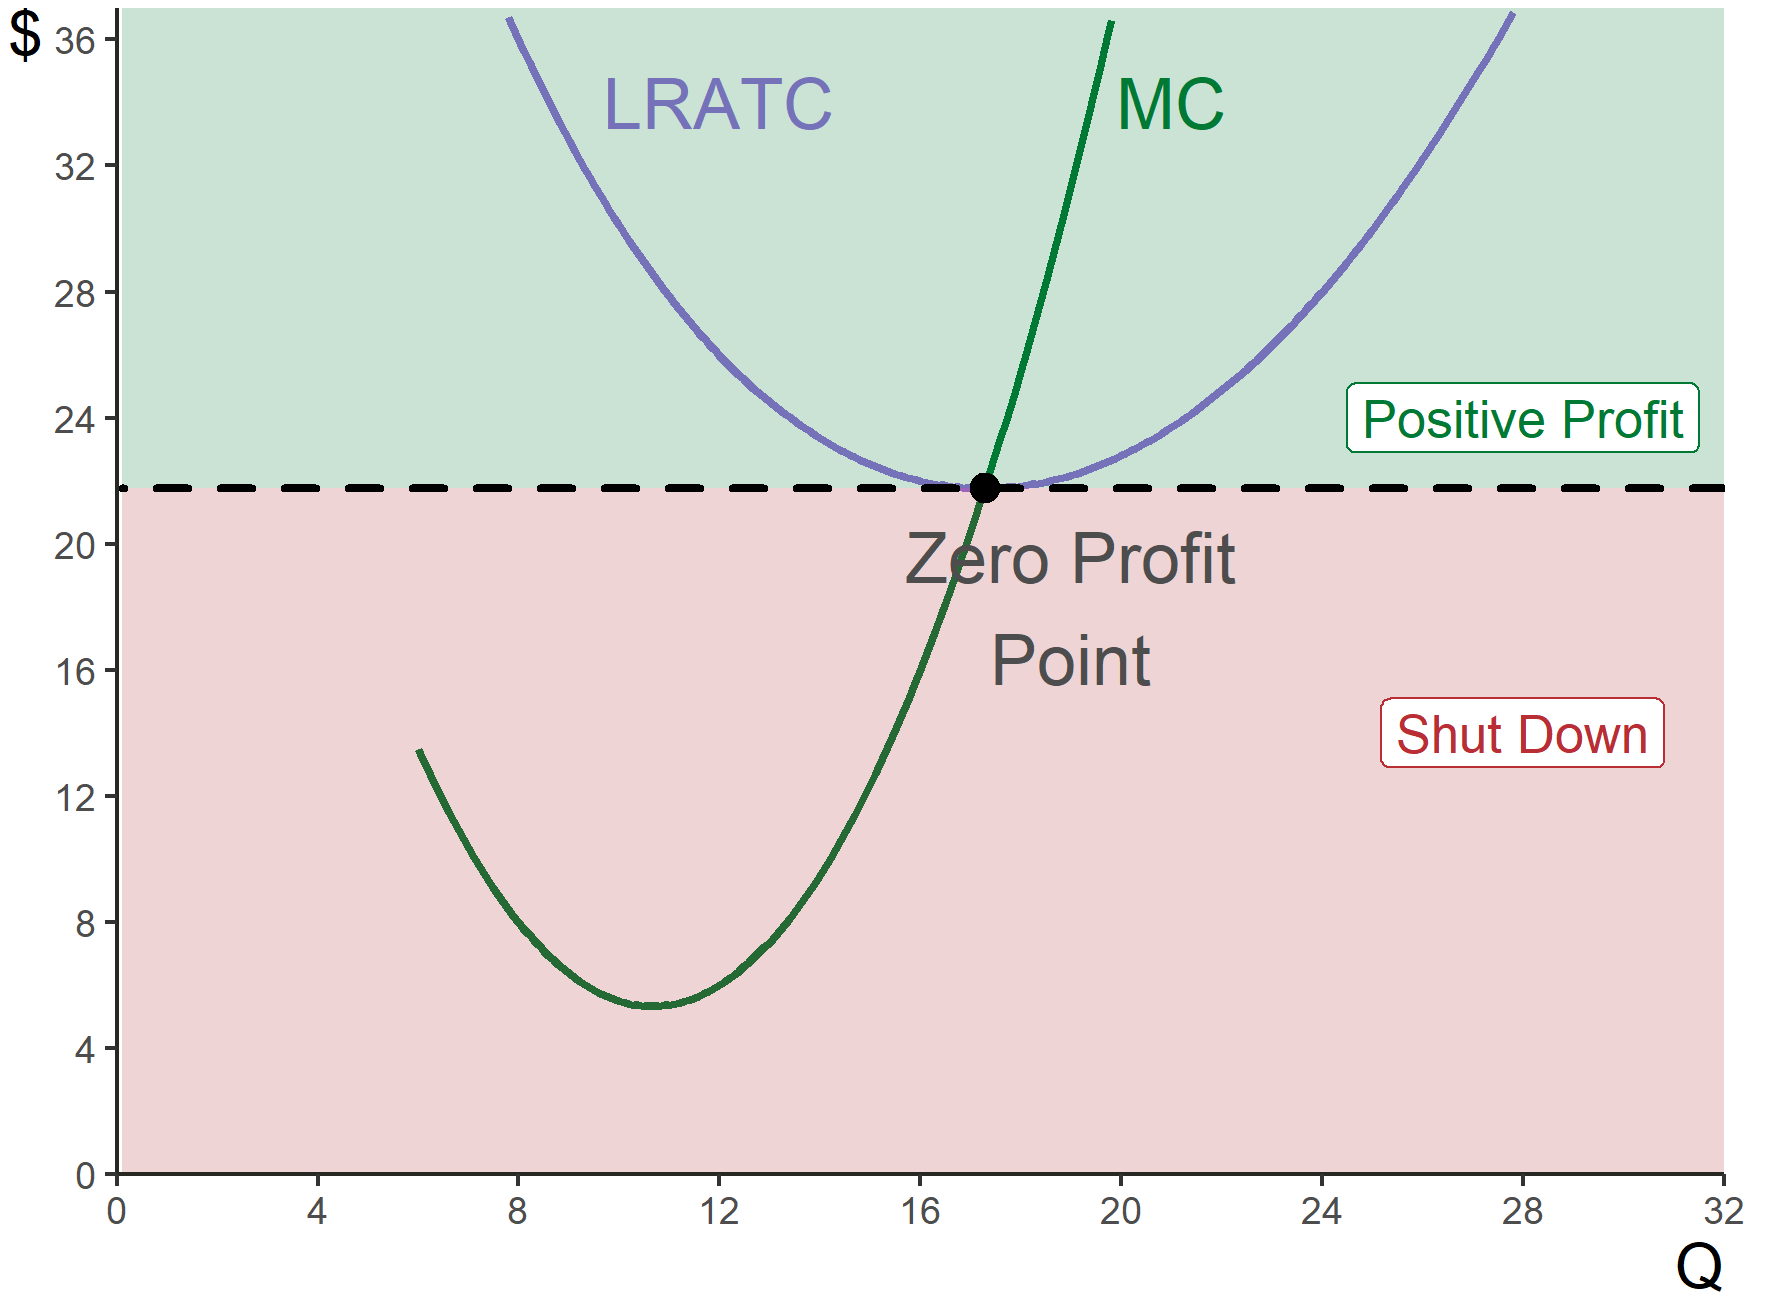
\includegraphics[width=7cm]{full shut.png}
        \end{figure}
    \end{itemize}
\end{frame}



\begin{frame}{Fun Fact}
    \begin{itemize}[<+->]
        \item This may be worth noting, but is not something I need you to memorize
        \begin{itemize}
            \item If TC is quadratic, MC and AVC are linear
            \item If AVC and MC are linear, then the firm will never shut down (more precisely, their shutdown condition will happen exactly when $Q=0$)
        \end{itemize}
        \item Example: suppose
        \begin{itemize}
            \item TC is given by $Q^{2}+6Q+10$
            \item MC is given by $2Q+6$
            \item AVC is given by $Q+6$
        \end{itemize}
        \item Let's graph MC and AVC and see what they look like
    \end{itemize}
\end{frame}

\begin{frame}{Fun Fact, Visualized}
    \begin{itemize}[<+->]
        \item The following firm should shut down when $P\le6$, but at this point, they would already be producing $Q\le 0$ (i.e. $Q=0$)
        \begin{figure}
            \centering
            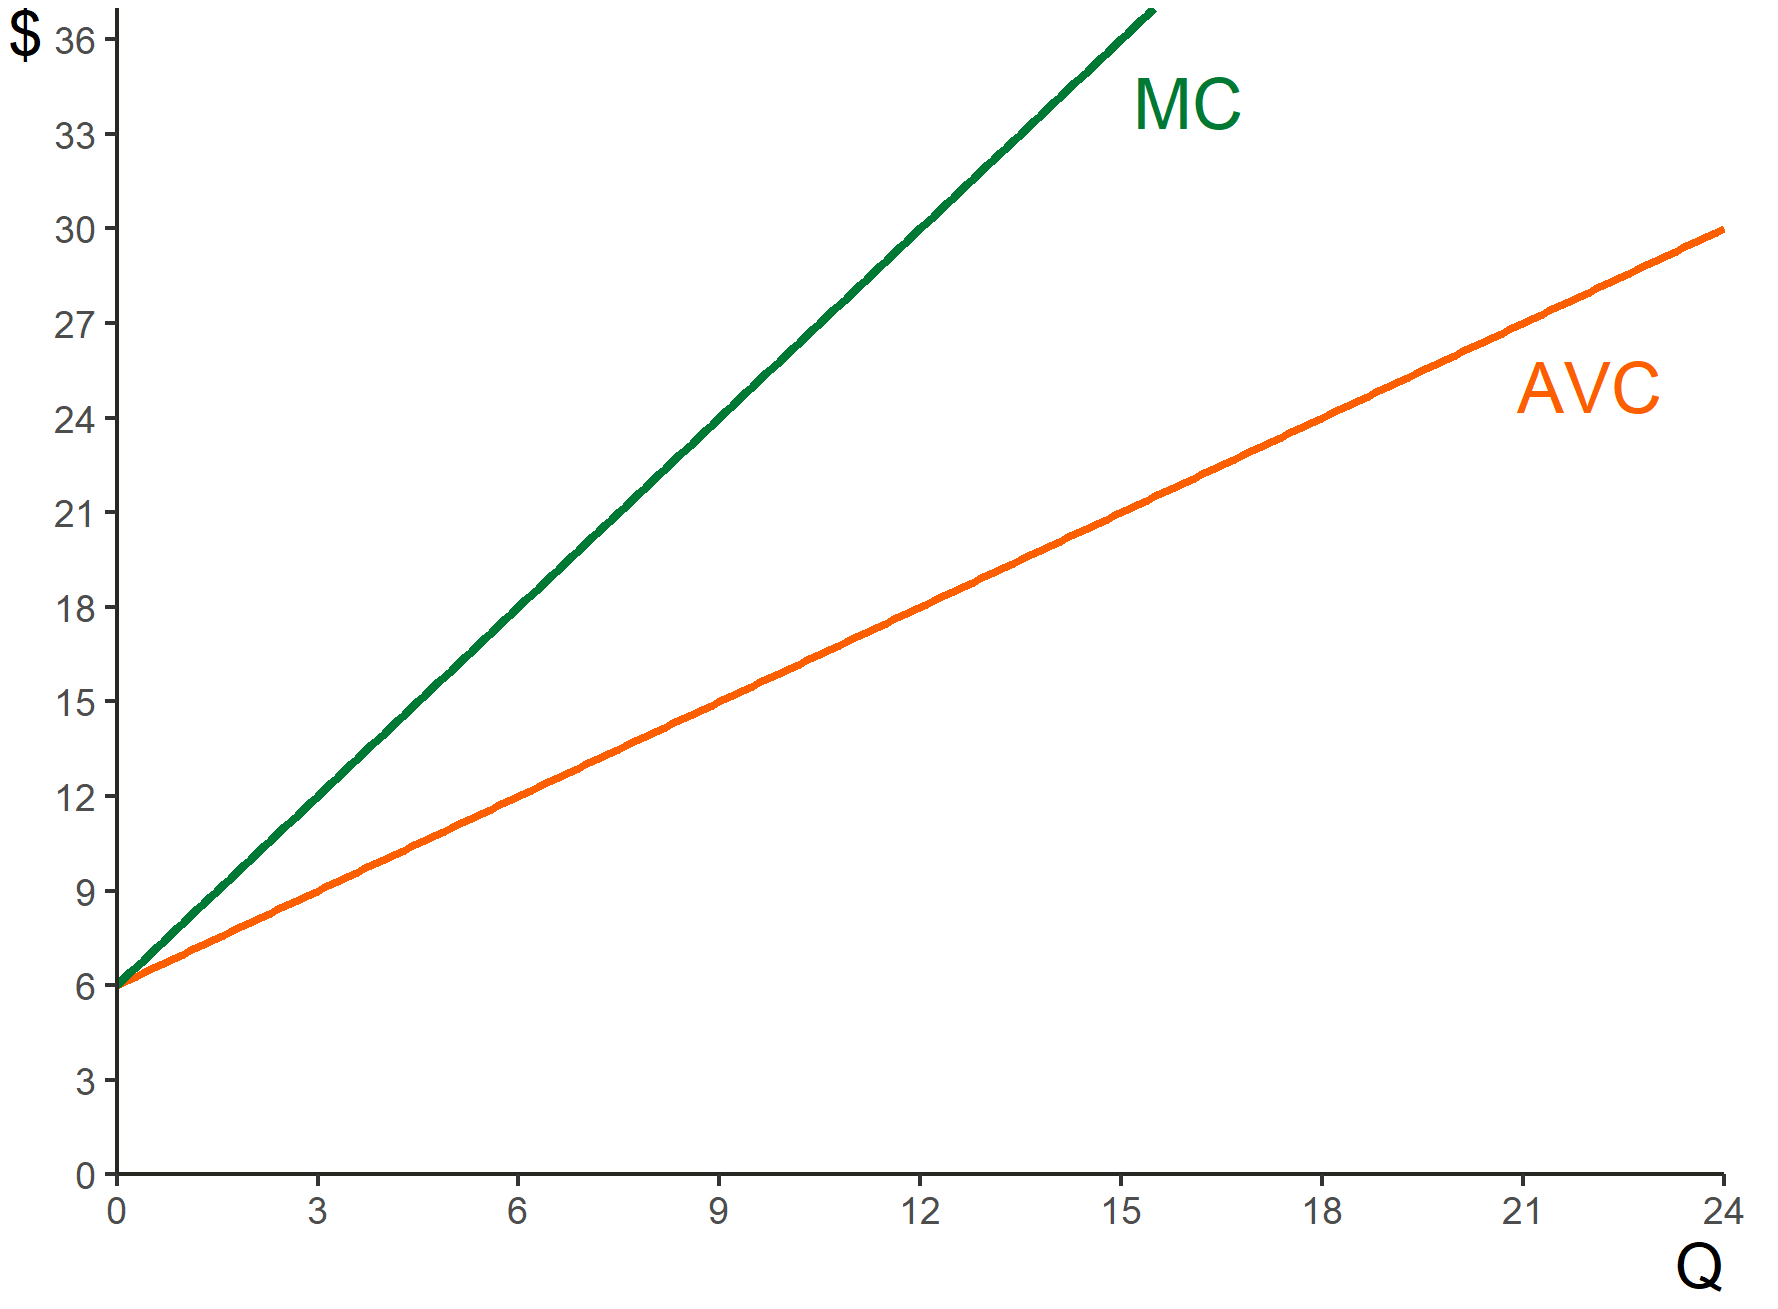
\includegraphics[width=7cm]{linear shut.png}
        \end{figure}
    \end{itemize}
\end{frame}

\begin{frame}{Shutting Down In the Long Run}
    \begin{itemize}[<+->]
        \item Recall: what are fixed costs in the long run?
        \begin{itemize}
            \item There aren't any
        \end{itemize}
        \item In the long run, AVC=ATC, so when should we shut down?
        \begin{itemize}
            \item When $P<\min(ATC)$ (specifically LRATC)
        \end{itemize}
        \item Idea: In the long run, when you are given full flexibility of all factors, you aren't covering your costs on average, you should leave the market
    \end{itemize}
\end{frame}


\begin{frame}{Shutting Down In the Long Run}
    \begin{itemize}[<+->]
        \item Here is the picture in the long run:
        \begin{figure}
            \centering
            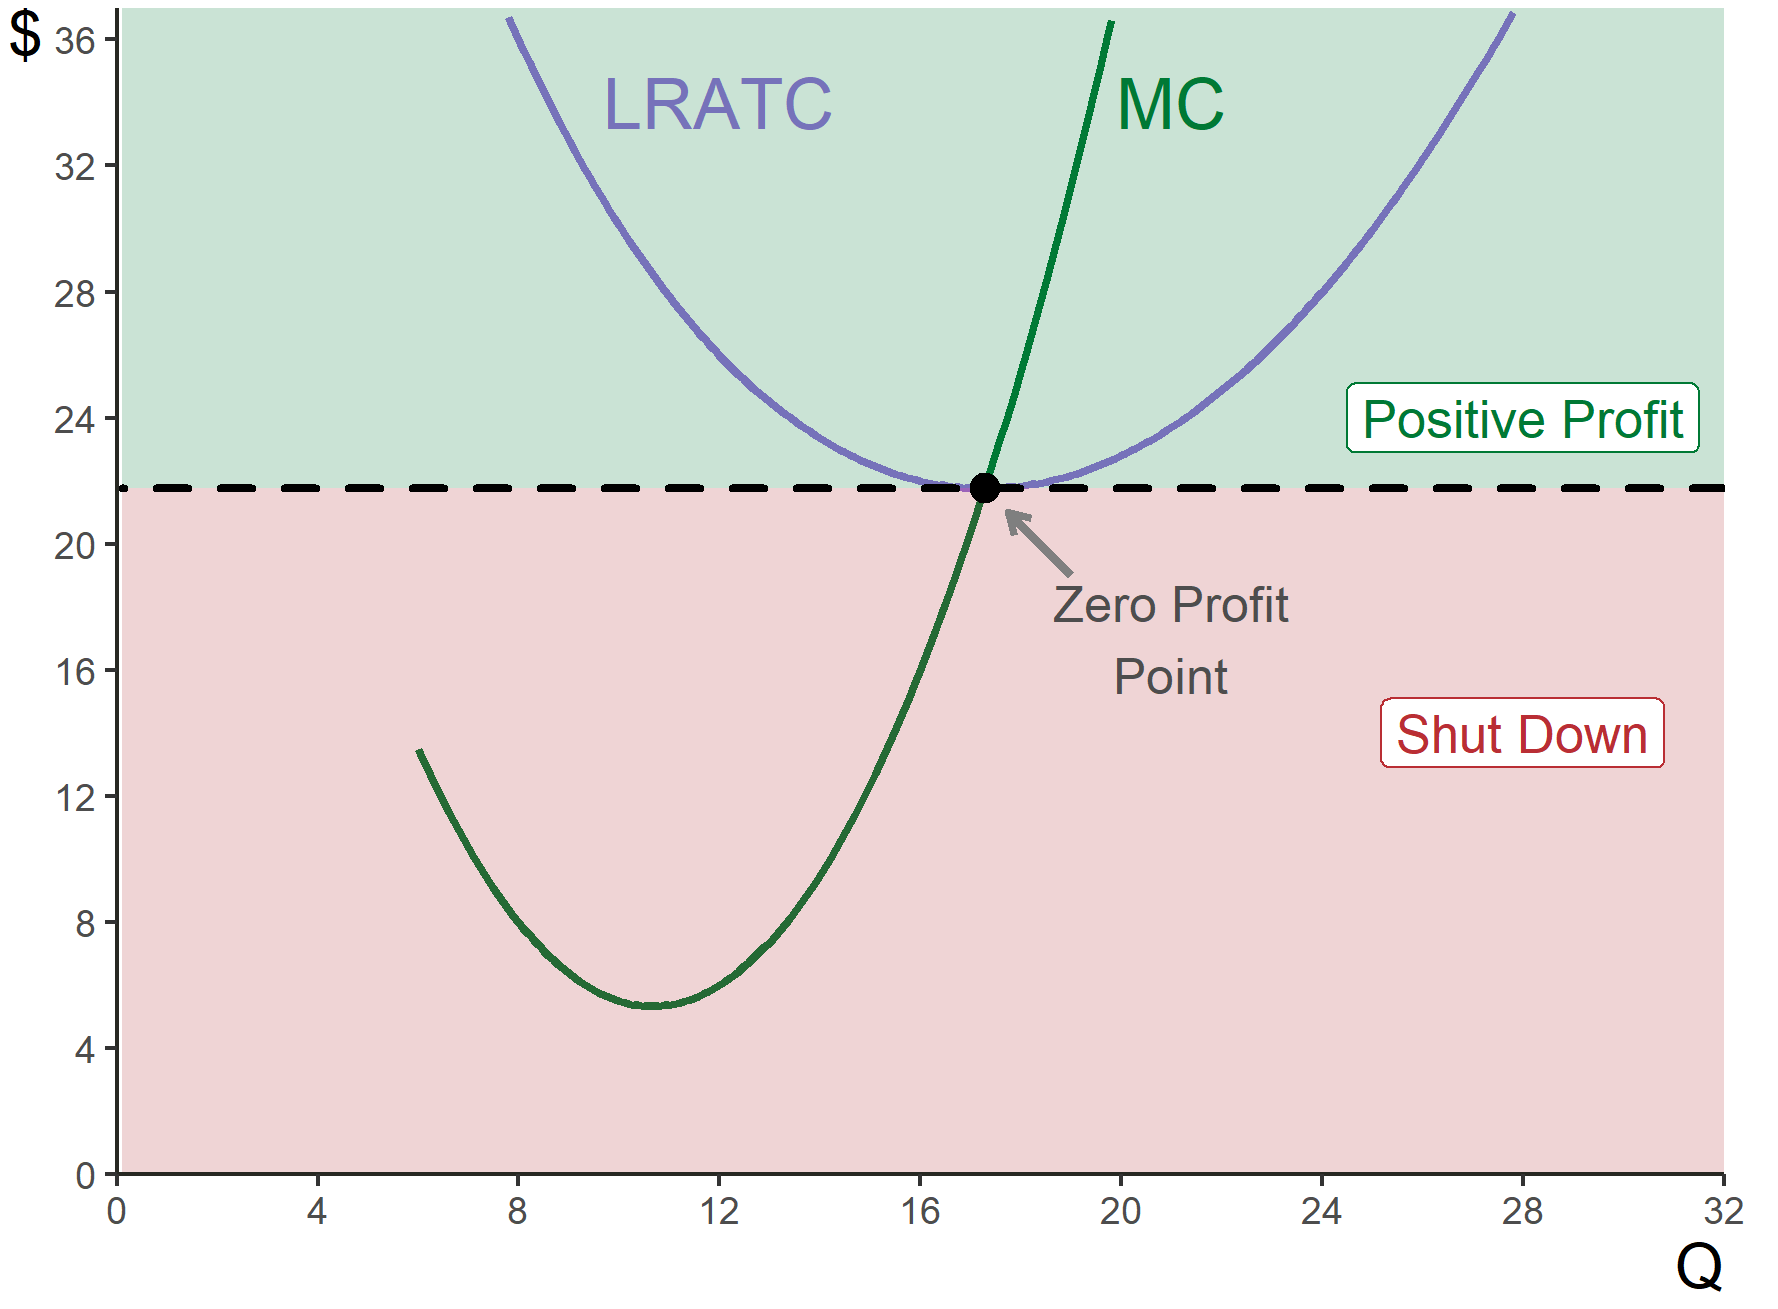
\includegraphics[width=7cm]{lr shut.png}
        \end{figure}
        \item Note: the zero profit point is also known as the break-even point
    \end{itemize}
\end{frame}





\section*{LR Profit}

\begin{frame}{What Happens When Firms Make Profits}
    \begin{itemize}[<+->]
        \item Let's suppose all of the firms in a PC market are making positive profits
        \item Recall: What kind of profits are we talking about?
        \begin{itemize}
            \item Economic: it's worth better than your best alternative
        \end{itemize}
        \item Firms are making positive economic profits and entry into the market is free. What do you think will happen?
        \begin{itemize}
            \item More firms will enter
        \end{itemize}
        \item What does more firms entering do to market supply? To price?
        \begin{itemize}
            \item Supply shifts right $\implies$ price moves down
        \end{itemize}
        \item How does a downward movement of price affect a PC firm's profits?
    \end{itemize}
\end{frame}

\begin{frame}{How $P\downarrow$ Affects a PC Firm's Profits}
    \begin{itemize}[<+->]
        \item A downward movement in price decreases a PC firm's profits:
        \vspace{5mm}
    \end{itemize}
        \makebox[\textwidth]{\vspace{10mm}
        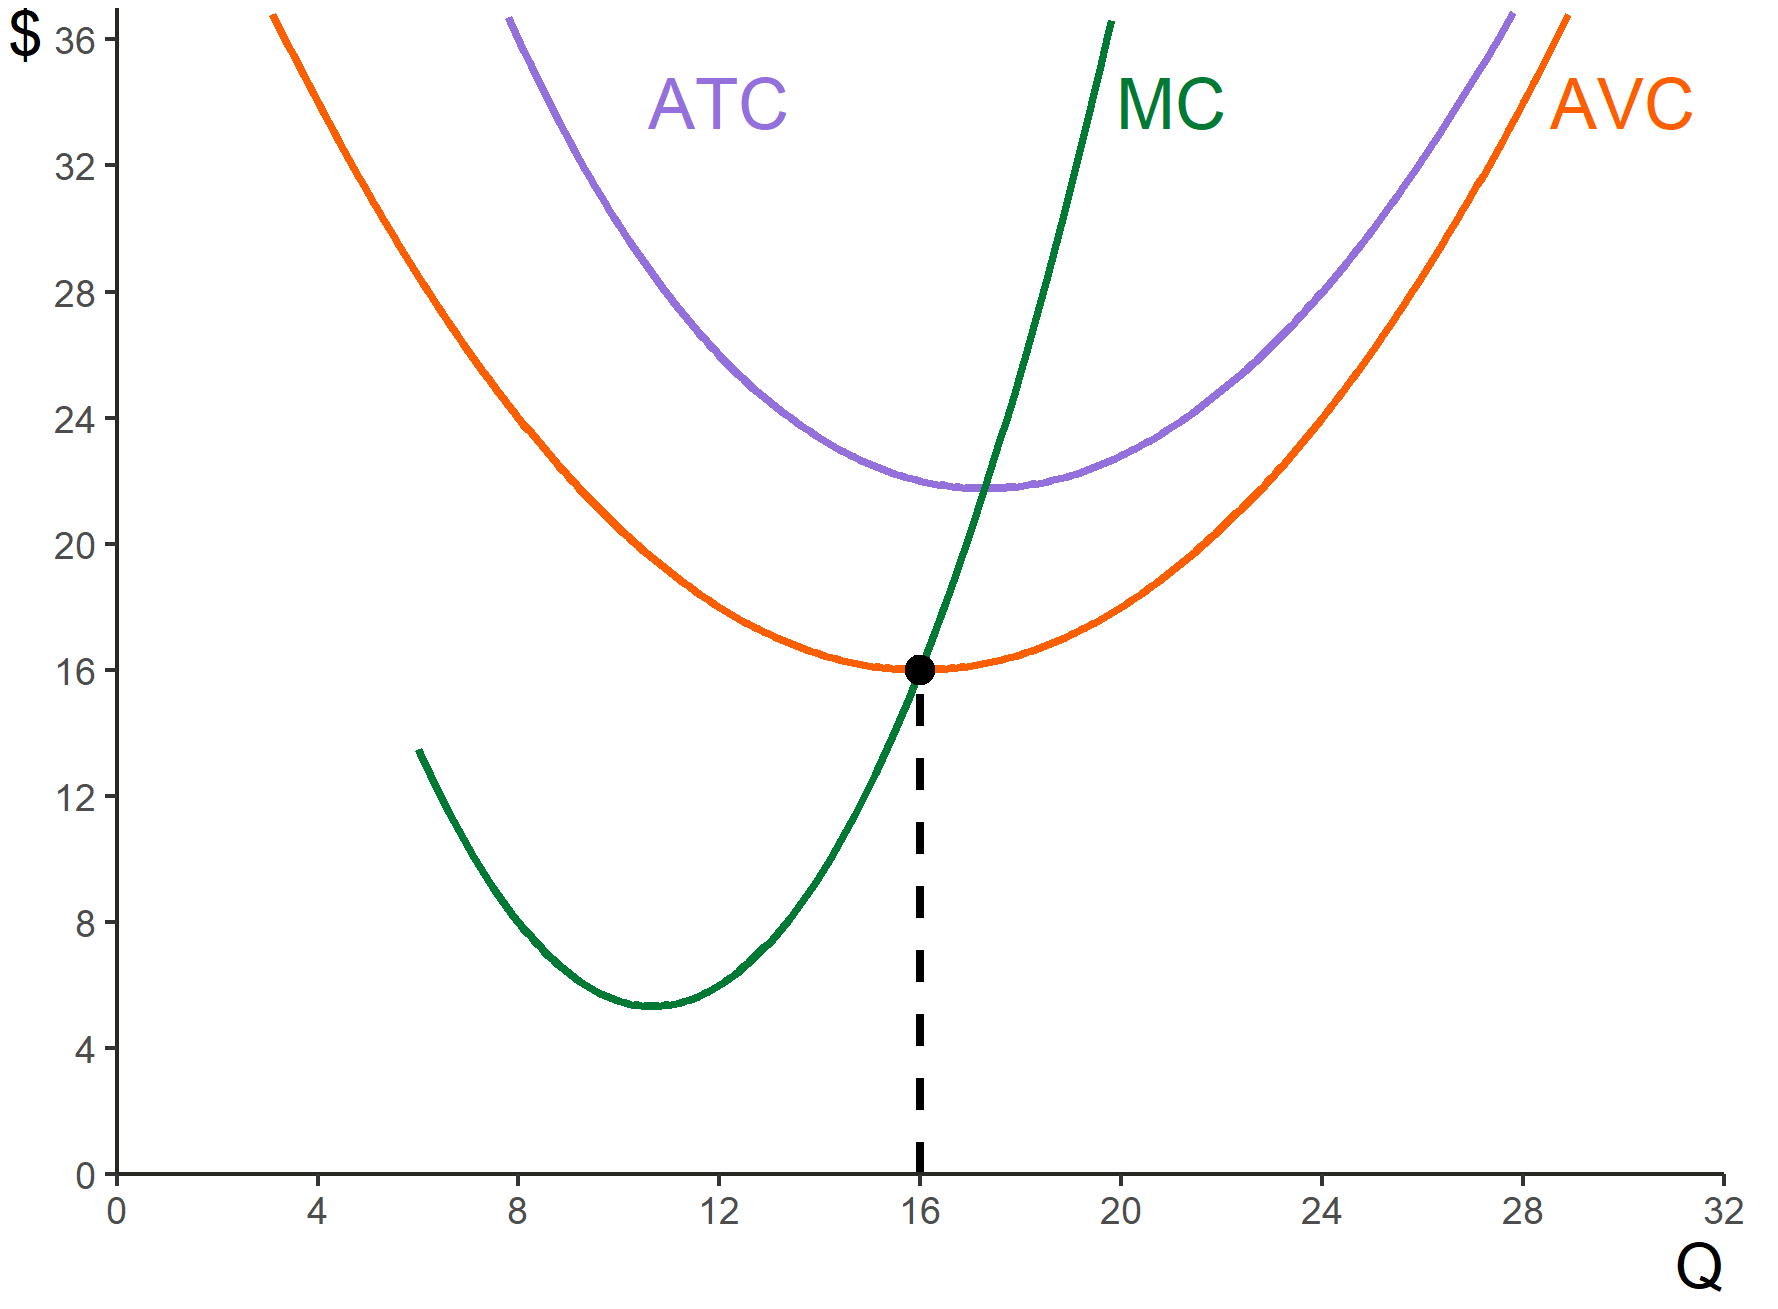
\includegraphics[width=0.48\paperwidth]{old profit.png}
        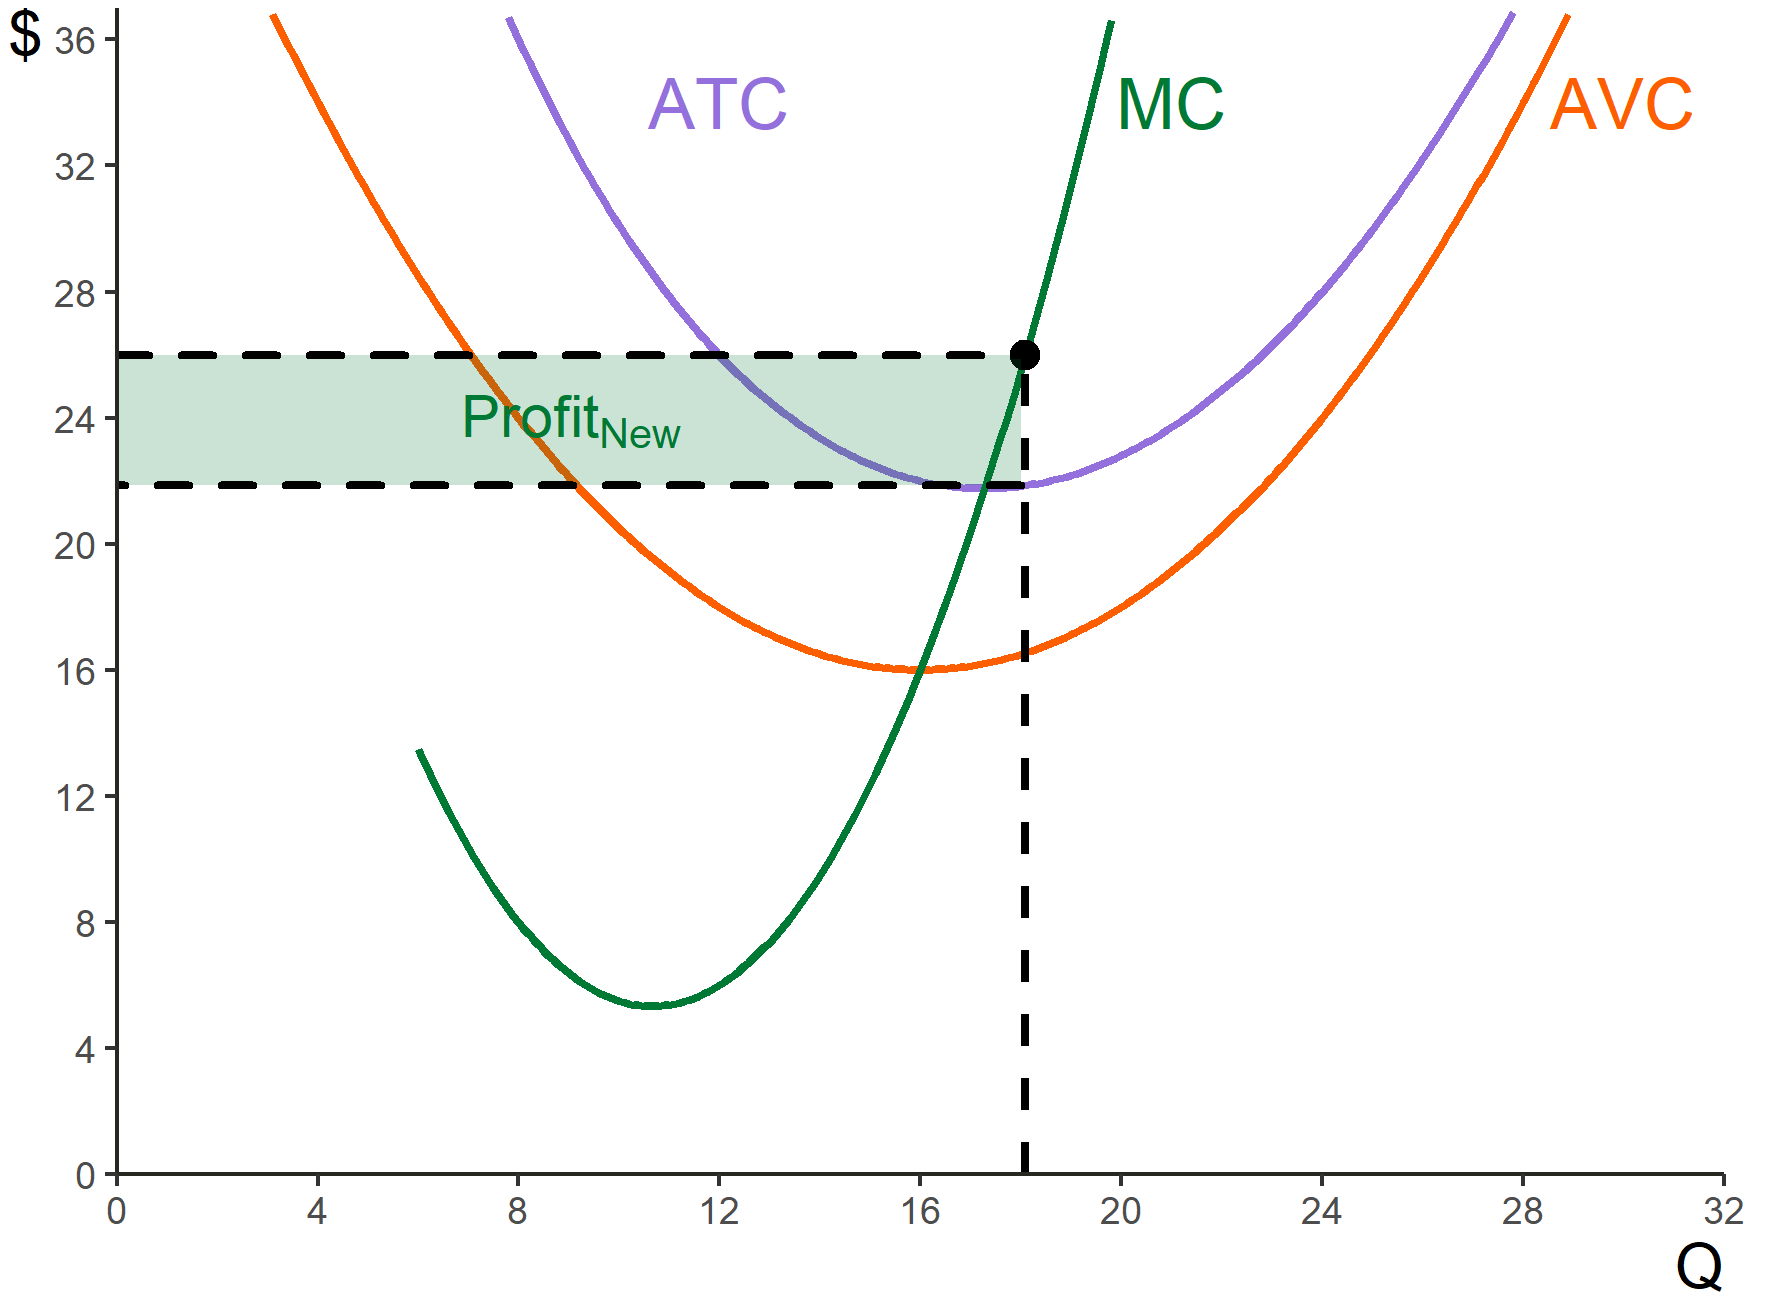
\includegraphics[width=0.48\paperwidth]{new profit.png}
        }
\end{frame}

\begin{frame}{What Happens When Firms Make Profits}
    \begin{itemize}[<+->]
        \item Let's suppose all of the firms in a PC market are \underline{still} making positive economic profits
        \begin{itemize}
            \item Rinse and repeat:
            \begin{itemize}
                \item More firms enter $\implies$ Price is driven down $\implies$ profits fall
            \end{itemize}
        \end{itemize}
        \item What happens if profits become negative?
        \begin{itemize}
            \item In the short run, firms will stay in business or shut down, depending on whether price is above or below $\min(AVC)$
            \item In the long run profits being negative means you leave the market entirely
            \item So, over time, the opposite happens:
            \begin{itemize}
                \item Firms leave the market $\implies$ supply shifts left $\implies$ price moves down $\implies$ profits rise
            \end{itemize}
        \end{itemize}
    \end{itemize}
\end{frame}

\begin{frame}{What Happens When Firms Make Profits}
    \begin{itemize}[<+->]
        \item Where do you think we end up?
        \item Result: in the long run, economic profit for perfectly competitive markets is \underline{\textit{zero}}
        \item This makes a lot of students uncomfortable: why would a firm stay in business if their long run profits are zero?
        \begin{itemize}
            \item Remember: economic profit
            \item This means that in the long run, the firm is not better or worse off doing anything else
        \end{itemize}
        \item \underline{Summary}
        \begin{itemize}
            \item In the short run, firms can make positive or negative profits, and may stay in the market with negative profits if they are covering their variable costs
            \item In the long run, firms in a PC market make zero profit: positive SR profits cause more firms to enter, driving down the price; negative profits eventually (in the LR) cause firms to leave, driving up the price
        \end{itemize}
    \end{itemize}
\end{frame}


\end{document}